% !TeX program = xelatex
%% 부득이하게 pdflatex을 사용해야 할 경우 위의 magic comment를 제거하십시오.

%%%%%%%%%%%%%%%%%%%%%%%%%%%%%%%%%%%%%%%%%%%%%%%%%%%%%%%%%%%%%%%%%%%%%%%%%%%%%%%%%
%%%  LaTeX document class of the thesis of the Gyeonggi Science High School   %%%
%%%  Last edition 2015.11.13 by Chinook Mok                                   %%%
%%%  Continously being modified by gshslatexintro after 2016.02.02.           %%%
%%%  Check the latest version at : latex.gs.hs.kr                             %%%
%%%  Also refer to https://www.facebook.com/gshstexsociety                    %%%
%%%%%%%%%%%%%%%%%%%%%%%%%%%%%%%%%%%%%%%%%%%%%%%%%%%%%%%%%%%%%%%%%%%%%%%%%%%%%%%%%

\documentclass{gshs_thesis}

\graphicspath{{images/}}
% 이곳에 필요한 별도의 패키지들을 적어넣으시오.
%\usepackage{...}
\usepackage{verbatim} % for commment, verbatim environment
\usepackage{spverbatim} % automatic linebreak verbatim environment
%\usepacakge{indentfirst}
\usepackage{tikz}
\usepackage{amsmath}
\usepackage{amsfonts}
\usepackage{amssymb}
\usepackage{float}
\usepackage{graphicx}

\usepackage{pgfplots}
\usetikzlibrary{shapes}
\usetikzlibrary{plotmarks}

\usepackage{listings}

\usepackage{hologo}
\usetikzlibrary{plotmarks}

\lstset{
	basicstyle=\small\ttfamily,
	columns=flexible,
	breaklines=true
}

\citation
\bibdata

%%%%%%%%%%%%%%%%%%%%%%%%%%%%%%%%%%%%%%%%%%%%%%%%%%%%%%%%%%%%%%%%%%%%%%%%%%   
% Define bar chart colors
%


% -----------------------------------------------------------------------
%                   이 부분은 수정하지 마시오.
% -----------------------------------------------------------------------
\titleheader{졸업논문청구논문}
\school{과학영재학교 경기과학고등학교}
\approval{위 논문은 과학영재학교 경기과학고등학교 졸업논문으로\\
졸업논문심사위원회에서 심사 통과하였음.}
\chairperson{심사위원장}
\examiner{심사위원}
\apprvsign{(인)}
\korabstract{초 록}
\koracknowledgement{감사의 글}
\korresearches{연 구 활 동}

%: ----------------------------------------------------------------------
%:                  논문 제목과 저자 이름을 입력하시오
% ----------------------------------------------------------------------
\title{SeaWiFS 해색 자료를 이용한 동해에서의 chlorophyll-a 농도 분석 : LAC 자료와 GAC 자료의 비교} %한글 제목
\engtitle{Analysis of the chlorophyll-a concentration in the East Sea (Sea of Japan) using SeaWiFS ocean color data : comparison between the LAC data and the GAC data} %영문 제목
\korname{김 병 현} %저자 이름을 한글로 입력하시오 (글자 사이 띄어쓰기)
\engname{Kim, Byung Hyun} %저자 이름을 영어로 입력하시오 (family name, personal name)
\chnname{金 柄 賢} %저자 이름을 한자로 입력하시오 (글자 사이 띄어쓰기)
\studid{15021} %학번을 입력하시오

%------------------------------------------------------------------------
%                  심사위원과 논문 승인 날짜를 입력하시오
%------------------------------------------------------------------------
\advisor{Park, Kie Hyun}  %지도교사 영문 이름 (family name, personal name)
\judgeone{박 경 애} %심사위원장
\judgetwo{김 학 성}   %심사위원1
\judgethree{박 기 현} %심사위원2(지도교사)
\degreeyear{2017}   %졸업 년도
\degreedate{2017}{11}{13} %논문 승인 날짜 양식

%------------------------------------------------------------------------
%                  논문제출 전 체크리스트를 확인하시오
%------------------------------------------------------------------------
\checklisttitle{[논문제출 전 체크리스트]} %수정하지 마시오
\checklistI{1. 이 논문은 내가 직접 연구하고 작성한 것이다.} %수정하지 마시오
% 이 항목이 사실이라면 다음 줄 앞에 "%"기호 삽입, 다다음 줄 앞의 "%"기호 제거하시오
\checklistmarkI{$\square$}
%\checklistmarkI{$\text{\rlap{$\checkmark$}}\square$}
\checklistII{2. 인용한 모든 자료(책, 논문, 인터넷자료 등)의 인용표시를 바르게 하였다.} %수정하지 마시오
% 이 항목이 사실이라면 다음 줄 앞에 "%"기호 삽입, 다다음 줄 앞의 "%"기호 제거하시오
\checklistmarkII{$\square$}
%\checklistmarkII{$\text{\rlap{$\checkmark$}}\square$}
\checklistIII{3. 인용한 자료의 표현이나 내용을 왜곡하지 않았다.} %수정하지마시오
% 이 항목이 사실이라면 다음 줄 앞에 "%"기호 삽입, 다다음 줄 앞의 "%"기호 제거하시오
\checklistmarkIII{$\square$}
%\checklistmarkIII{$\text{\rlap{$\checkmark$}}\square$}
\checklistIV{4. 정확한 출처제시 없이 다른 사람의 글이나 아이디어를 가져오지 않았다.} %수정하지 마시오
% 이 항목이 사실이라면 다음 줄 앞에 "%"기호 삽입, 다다음 줄 앞의 "%"기호 제거하시오
\checklistmarkIV{$\square$}
%\checklistmarkIV{$\text{\rlap{$\checkmark$}}\square$}
\checklistV{5. 논문 작성 중 도표나 데이터를 조작(위조 혹은 변조)하지 않았다.} %수정하지 마시오
% 이 항목이 사실이라면 다음 줄 앞에 "%"기호 삽입, 다다음 줄 앞의 "%"기호 제거하시오
\checklistmarkV{$\square$}
%\checklistmarkV{$\text{\rlap{$\checkmark$}}\square$}
\checklistVI{6. 다른 친구와 같은 내용의 논문을 제출하지 않았다.} %수정하지 마시오
% 이 항목이 사실이라면 다음 줄 앞에 "%"기호 삽입, 다다음 줄 앞의 "%"기호 제거하시오
\checklistmarkVI{$\square$}
%\checklistmarkVI{$\text{\rlap{$\checkmark$}}\square$} % usepackage 등의 명령어는 여기에.

\usepackage{tocloft}
\setlength{\cftbeforesecskip}{0pt}
\setlength{\cftbeforesubsecskip}{0pt}
\setlength{\cftbeforesubsubsecskip}{0pt}

\begin{document}
%	\renewcommand\baselinestretch{1.2} % line spacing in the paragraph
	\baselineskip=2.2em         % line spacing in the paragraph
	
	\maketitle  % command to print the title page with above variables

\setcounter{page}{1}
%---------------------------------------------------------------------
%                  영문 초록을 입력하시오
%---------------------------------------------------------------------
\begin{abstracts}     %this creates the heading for the abstract page
	\addcontentsline{toc}{section}{Abstract}  %%% TOC에 표시
	\noindent{
		다시 번역
		The seasonal variability chlorophyll-a concentration in the Korean East Sea had been obtained by processing SeaWiFS Local Area Coverage(LAC) and Global Area Coverage(GAC) oceancolor data from January 2003 to December 2006. Both data showed similarities in the tendency showing peaks on spring(April) and fall(November). However, the value of chlorophyll-a concentration was different, the maximum/minimum value of LAC and GAC data each being 1.61 mg/m3 / 0.28 mg/m3, and 1.72 mg/m3 / 0.32 mg/m3. Comparing the pixel histogram of LAC and GAC data showed GAC data had more speckle errors. The pixel analysis of chlorophyll-a concentration data on April, 2003 also showed it is more accurate to use LAC data because of its high resolution.
	}
\end{abstracts}

%---------------------------------------------------------------------
%                  국문 초록을 입력하시오
%---------------------------------------------------------------------
\begin{abstractskor}        %this creates the heading for the abstract page
	\addcontentsline{toc}{section}{초록}  %%% TOC에 표시
	\noindent{
SeaWiFS LAC (Local Area Coverage) 및 GAC (Global Area Coverage) 자료를 이용하여 2003년 1월부터 2006년 12월까지 동해의 chlorophyll-a 월평균 농도를 산출하였다. 두 자료 모두 봄철(4월)과 가을철(11월)에 월평균 농도가 높게 산출되어 전체적인 경향은 비슷하게 나타났다. 그러나 LAC와 GAC 자료로 산출한 chlorophyll-a 월평균 농도의 최대값/최소값은 각각 1.61 $\rm mg/m^3$ / 0.28 $\rm mg/m^3$ 과 1.72 $\rm mg/m^3$ / 0.32 $\rm mg/m^3$으로 차이가 나타났다. 차이를 구체적으로 분석하기 위하여 LAC와 GAC 데이터의 픽셀 히스토그램을 비교한 결과 GAC 데이터에서 스펙클 오류가 더 크게 나타남을 확인하였다. Chlorophyll-a 월평균 농도가 높았던 2003년 4월 이미지 픽셀을 분석해 본 결과 해상도가 높은 LAC 자료를 이용하는 것이 GAC 자료를 이용하는 것 보다 더 정확함을 확인하였다. 
	}
\end{abstractskor}

%----------------------------------------------
%   Table of Contents (자동 작성됨)
%----------------------------------------------
\cleardoublepage
\addcontentsline{toc}{section}{Contents}
\setcounter{secnumdepth}{3} % organisational level that receives a numbers
\setcounter{tocdepth}{3}    % print table of contents for level 3
\baselineskip=2.2em
\tableofcontents


%----------------------------------------------
%     List of Figures/Tables (자동 작성됨)
%----------------------------------------------
\cleardoublepage
\clearpage
\listoftables
% 표 목록과 캡션을 출력한다. 만약 논문에 표가 없다면 이 위 줄의 맨 앞에 
% `%' 기호를 넣어서 주석 처리한다.

\cleardoublepage
\clearpage
\listoffigures
% 그림 목록과 캡션을 출력한다. 만약 논문에 그림이 없다면 이 위 줄의 맨 앞에 
% `%' 기호를 넣어서 주석 처리한다.

\cleardoublepage
\clearpage
\listofequations
% 그림 목록과 캡션을 출력한다. 만약 논문에 그림이 없다면 이 위 줄의 맨 앞에 
% `%' 기호를 넣어서 주석 처리한다.


\cleardoublepage
\clearpage
\renewcommand{\thepage}{\arabic{page}}
\setcounter{page}{1} % Abstract

	%%%%%%%%%%%%%%%%%%%%%%%%%%%%%%%%%%%%%%%%%%%%%%%%%%%%%%%%%%%
	%%%% Main Document %%%%%%%%%%%%%%%%%%%%%%%%%%%%%%%%%%%%%%%%
	%%%%%%%%%%%%%%%%%%%%%%%%%%%%%%%%%%%%%%%%%%%%%%%%%%%%%%%%%%%

	\section{Introduction}

Ocean color remote sensing allows the indirect measurement of various matters in the ocean. The Coastal Zone Color Scanner (CZCS) is the first ocean color sensor, operated from 1978 to 1986 and the Sea-viewing Wide Field-of-view Sensor (SeaWiFS) has observed global ocean color distributions for about a decade, from 1998 to 2010, and has provided the scientific community with abundant information for a variety of oceanic application research \cite{kyung2013characteristics, hooker1992An}. Ocean color remote sensing is executed by collecting several bands of reflected light from the ocean and calculating the collected data to amount of matters in water using the algorithms developed through. Such data collected through this method is called ocean color data. Ocean color data is important in understanding the temporal and spatial distribution of algae \cite{kimhc2016surface}.

Chlorophyll-a concentration can be calculated using ocean color remote sensing. Since chlorophyll-a is a pigment that is required in photosynthesis, it is also found in algae. Additionally, chlorophyll-a concentration is used as a determinant for the amount of algae in ocean \cite{o2000ocean}. 

There have been several studies about chlorophyll-a concentration in the East Sea using ocean color remote sensing. The chlorophyll-a concentration was found to be related with wind, sea surface temperature, and many other variables of the ocean. Spring bloom and fall bloom were observed in the East Sea, showing a seasonal pattern \cite{yamada2004seasonal}. SeaWiFS satellite is often used for studying the chlorophyll-a concentration in the East Sea. It was found out that some of the area had abnormally higher concentration of chlorophyll-a compared to the areas nearby. These areas are called speckles. Speckles are errors made by SeaWiFS, so there had been studies to correct them. \cite{chae2009characteristics}. 

SeaWiFS creates two types of data with different spatial resolutions, Local Area Coverage (LAC) data and Global Area Coverage (GAC) data. LAC data is created with full-resolution (1.1 $\rm km$) for local area by combining the continuously recorded images. On the other hand, GAC data is created with low resolution (4.5 $\rm km$) subsampled from the full-resolution data with every fourth pixel to show a global area \cite{Seawifsres}. 

Although many scientists used SeaWiFS LAC data and GAC data for research, they did not found which data is more suitable. Which data is more accurate There is also no proof that applying the same algorithms gives the same accurate results. Thus, the difference between LAC data and GAC data should be discussed. 

The goals of this research are the followings. First, observing the chlorophyll-a concentration variability in the East Sea from 2003 to 2006 using SeaWiFS ocean color data. Second, comparing the chlorophyll-a concentration data of LAC and GAC to find the effect of spatial resolution. The monthly mean data were compared and the differences of the data were calculated. Also, pixels over 10 $\rm mg~m^{-3}$ were analysed. The maximum value of each month were also compared. These researches were conducted to find out which data is more reliable.
 % Introduction
	\section{Methodology}

\subsection{Study area}

<<<<<<< HEAD
The East Sea (Sea of Japan) was chosen to calculate chlorophyll-a concentration using the ocean color data. The study area is shown in Figure \ref{fig:Map_of_Research_Area}. as 34.00°N - 44.00°N, 127.°E - 135.00°E which covers the whole East Sea (Sea of Japan) near Korea. The South Sea and the Yellow Sea was excluded from the study area because it is difficult to calculate the chlorophyll-a concentration using the ocean color algorithm due to their shallow depth. 

The depth of the East Sea rapidly increases from the east coast. The East has a surface area of about 978,000 $\rm km^2$, a mean depth of 1,752 $\rm m $ and a maximum depth of 3,742 $\rm m$. Such depth allows to use the developed chlorophyll-a algorithms. Terrains under the East Sea near Korean Peninsula is complex and the area of the continental shelf is steep.

\begin{figure}[h]

	\centering
{\includegraphics[width=0.95\textwidth]	{Map_of_Research_Area} }

\caption{Map showing study area.}
	\label{fig:Map_of_Research_Area}

\end{figure}

\newpage


\subsection{SeaWiFS data and Study period}

SeaWiFS ocean color data is used in order to calculate chlorophyll-a concentration of the East Sea (Sea of Japan) in this study. However, it is not able to obtain recent measurements since SeaWiFS had only activated from September 1997 to December 2010. {Table \ref{table01}.} shows the mission charactoristics of SeaWiFS and Table \ref{table02} shows the Cahracteristics of the SeaWiFS ocean color sensor \cite{hooker1992An}.

 \begin{table}[h]%[width=1.0\linewidth]
 	\caption{The mission characteristics of SeaWiFS.}
 	\label{table01}
 	\centering
 	\begin{tabular}{c|c}
 		\hline \setlength{\arrayrulewidth}{0.8pt}. 
 	Orbit Type	& Sun Synchronous at 705 km \\ \hline
 	Equator Crossing &	Noon +20 min, descending \\ \hline
 	Orbital Period &	99 minutes  \\ \hline
 	Swath Width &	2,801 km LAC/HRPT (58.3 degrees)  \\ \hline
 	Swath Width &	1,502 km GAC (45 degrees)  \\ \hline
 	Spatial Resolution &	1.1 km LAC, 4.5 km GAC  \\ \hline
 	Real-Time Data Rate &	665 kbps  \\ \hline
 	Revisit Time &	1 day  \\ \hline
 	Digitization &	10 bits  \\ \hline
 	\end{tabular}
 \end{table}

 \begin{table}[h]%[width=1.0\linewidth]
	\caption{Cahracteristics of the DeaWiFS ocean color sensor.}
	\label{table02}
	\centering
	\begin{tabular}{c|c|c|c|c}
		\hline \setlength{\arrayrulewidth}{0.8pt}. 
		Band	& Wavelength FWHM[nm] & Saturation Radiance & Input Radiance & SNR\\ \hline{5.0pt}
		1 & 402-422 & 13.63 & 9.10 & 499 \\ \hline
		2 & 433-453 & 13.25 & 8.41 & 674  \\ \hline
		3 & 480-500 & 10.50 & 6.56 & 667 \\ \hline
		4 & 500-520 & 9.08 & 5.64 & 640  \\ \hline
		5 & 545-565 & 7.44 & 4.57 & 596 \\ \hline
		6 & 660-680 & 4.20 & 2.46 & 442  \\ \hline
		7 & 745-785 & 3.00 & 1.61 & 455 \\ \hline
		8 & 845-885 & 2.13 & 1.09 & 467  \\ \hline
	\end{tabular}
\end{table}
 
 The Ocean Biology Processing Group collects and processes data from Earth-viewing satellites. These data are organized in various ways reflecting different spatial, temporal, and parameter groupings. Over the years, certain terminology about remote sensing data has arisen to describe these organizational conventions. Level-0 is unprocessed data from remote sensing instruments at a full resolution. Level-1 data is obtained through radiometric and geometric calibration. Level-2 data is made of geophysical variables processed from level-1 data using developed algorithms \cite{feldman2017ocean}. In this research, chlorophyll-a concentration is the geophyscial variable we choose to process.


The SeaWiFS Level-2 Ocean Color chlorophyll-a Data Version 2014 can be downloaded from the NASA Goddard Space Flight Center (GSFC) Distributed Active Archive Center (DAAC). Processing Level-1 data to Level-2 data was conducted by NASA, using NASA SeaDAS program\cite{NASASeaFiWSdata}. NASA SeaDAS uses two algorithms to create chlorophyll-a concentration data from the Level-1 data of remote sensing reflectance ($\rm R_{rs}$); these algorithms are the OCx band ratio algorithm and the color index (CI) algorithm of Hu. 
 The OCx band ratio algorithm use the ratio of two bands in a fourth-order polynomial equation in a relation with chlorophyll-a. It can be expressed as \eqref{eq:001}.
 
 \begin{equation}
 {\rm log_{10} (chlor_a) = a_0 + \sum_{i=1}^4 a_i ~ log_{10} \left( \frac{(R_{rs}(\lambda_{blue})}{(R_{rs}(\lambda_{green})} \right) ^i }
 \label{eq:001}
 \end{equation}
 
The coefficients $\rm a_0$ - $\rm a_4$ are values for each sensor acquired experimentally. The OCx algorithm was proved to be accurate by O’Reilly et. al\cite{o2000ocean}. The CI algorithm uses three bands and can be expressed as \eqref{eq:002}.

 \begin{equation}
{\rm CI = R_rs ({\lambda}_{green}) - [R_rs ({\lambda}_{blue}) + \frac {({\lambda}_{green}) - {\lambda}_{blue})} {({\lambda}_{red}) - {\lambda}_{blue}} * ({\lambda}_{red}) - R_rs ({\lambda}_{blue}) ]}
\label{eq:002}
\end{equation}

The $\rm {\lambda}_{blue}$, $\rm {\lambda}_{green}$, $\rm {\lambda}_{red}$ are wavelengths closest to 443 $\rm nm$, 555 $\rm nm$ and 670 $\rm nm$, different for each sensor. According to Hu, C., Lee, Z., and Franz, B., for the lower concentration of chlorophyll-a (less than 0.25 $\rm mg/m^3$), it is more accurate to use CI algorithm \cite{hu2012chlorophyll}. The NASA SeaDAS software uses CI algorithm for chlorophyll retrievals below 0.15 $\rm mg/m^3$, and OCx band ratio algorithm for retrievals above 0.2 $\rm mg/m^3$. For the concentration between 0.15 $\rm mg/m^3$ and 0.2 $\rm mg/m^3$, it blends both algorithm.

The level-2 GAC data of the East sea (Sea of Japan) can be obtained from 1997 to 2010 but the level-2 LAC data can be obtained only from 2003 to 2006. Only a few LAC data files of the East Sea (Sea of Japan) are available after 2007. That is why the study period was set from 2003 to 2006. The information of on used data is shown in Table \ref{data_information}.
The level-3 LAC and GAC data are derived geophysical variables that have been aggregated onto a well-defined over a well-defined time period and projected onto a well-defined spatial grid.

start 박기현 추가
 \begin{table}[h]
	\caption{The number of Level-2 files for analysis.}
	\label{data_information}
	\centering
	\begin{tabular}{c | c | c }
		\hline \setlength{\arrayrulewidth}{3.5pt}. 
			& LAC  & GAC \\ \hline
		2003 (N) & 482 & 490 \\ \hline
		2004 (N) & 441 & 497 \\ \hline
		2005 (N) & 270 & 494 \\ \hline
		2006 (N) & 313 & 498 \\ \hline
		total (N) & 1,506 & 1,979 \\ \hline
	\end{tabular}
\end{table}
end 박기현추가

\hfill \break
\hfill \break


 \subsection{Deriving Chlorophyll-a Concentration using LAC data and GAC data}
 
NASA SeaDAS is used to process the level-2 data of chlorophyll-a to level-3 data of monthly-mean/ 8-day-mean of chlorophyll-a concentration data. Monthly-mean data is created to show the overall tendency, while 8-day-mean data is created to see more specific tendency. Simple average method had been used to create the mean files. This method sums pixel values of chlorophyll-a at the same location and divides it by the number of data that have been compiled. This process also gives latitude longitude value to the pixels, creating a Standard Mapped Image (SMI). Chae, H. J., \& Park, K. (2009) used weighted average method to process data. However, according to Park, K. A., Park, J. E., Lee, M. S., \& Kang, C. K. (2012), both the weighted average method and the simple average method are suitable for processing SeaWiFS data in the East Sea (Sea of Japan). In addition, the more general method, the simple average method is used in this research.
  
 Since running each process using SeaDAS is inconvenient, so the process is automated by using python batch processing. This commands SeaDAS to repeat the process. Python can also create png files from the SMI. We use the obtained monthly-mean and 8-day-mean data to find the annual variability of chlorophyll-a concentration.
 
 The effect of spatial resolution on the data was studied by comparing the LAC and the GAC data. The monthly average data was compared and the differences of the values were calculated. Further analysis was done on pixels with a value over 10 $\rm mg/m^3$. The maximun value of each month was also compared. These research were done to find out which data showed more accuracy and precision
 
 	
%	
\section{Results}
 
\subsection{The Annual Variability of Chlorophyll-a Concentration in the Korean East Sea}
 
The annual variability of chlorophyll-a concentration in the Korean East Sea from 2003 - 2006 is shown in Figure 1, Figure 2. Both the LAC data and the GAC data has similar tendency, showing peaks on spring(April) and fall(November). The maximum/minimum value of LAC and GAC data was each 1.61 mg/m3 / 0.28 $\rm mg/m^3$, and 1.72 $\rm mg/m^3$ / 0.32 $\rm mg/m^3$. The difference between the two data was not ignorable. This infer that the effect of spatial resolution on the data has to be considered.
  
 Figure.
 
The annual variability of 8-day-mean chlorophyll-a concentration in the Korean East Sea from 2003 to 2006 is shown in Figure 3, Figure 4. This result allowed more concrete analysis of the data. The spring peak had 1.2 ~ 1.3 $\rm mg/m^3$ of chlorophyll-a concentration and was higher than the fall peak which had the value of 0.9 ~ 1.0 $\rm mg/m^3$. Winter had a higher concentration (0.6 $\rm mg/m^3$) compared to summer (0.4 $\rm mg/m^3$). The chlorophyll-a concentration in the Korean East Sea had clear seasonal differences. Both the LAC data and the GAC data was sufficient to show the seasonal differences. However, even though the 8-day mean data was created using average of 4 years, the time of maximum concentration was different. 

Part of the LAC data (2004 46th 8-day mean, 2005 11th 8-day mean, 2005 31th 8-day mean) had been lost due to satellite failures. The data for these dates were substituted with the average of the adjacent data. This did not have a significant effect on the tendency, so the error was ignorable.
  
  Figure.
 
The monthly-mean chlorophyll-a concentration of LAC from 2003 to 2006 is shown in \ref{fig:noname01} and \ref{fig:noname02}. The monthly-mean chlorophyll-a concentration of GAC from 2003 to 2006 is shown in \ref{fig:noname03} and \ref{fig:noname04}. The grey area is land showing Korea at the west and Japan at the southeast. Red means high concentration than the blue as it can be told from the color bar. Spring (March, April, May) and fall (October, November) show high concentration. The black area is part with no data due to cloud coverage or satellite failures. 
    
\begin{figure}[t]
	\centering
	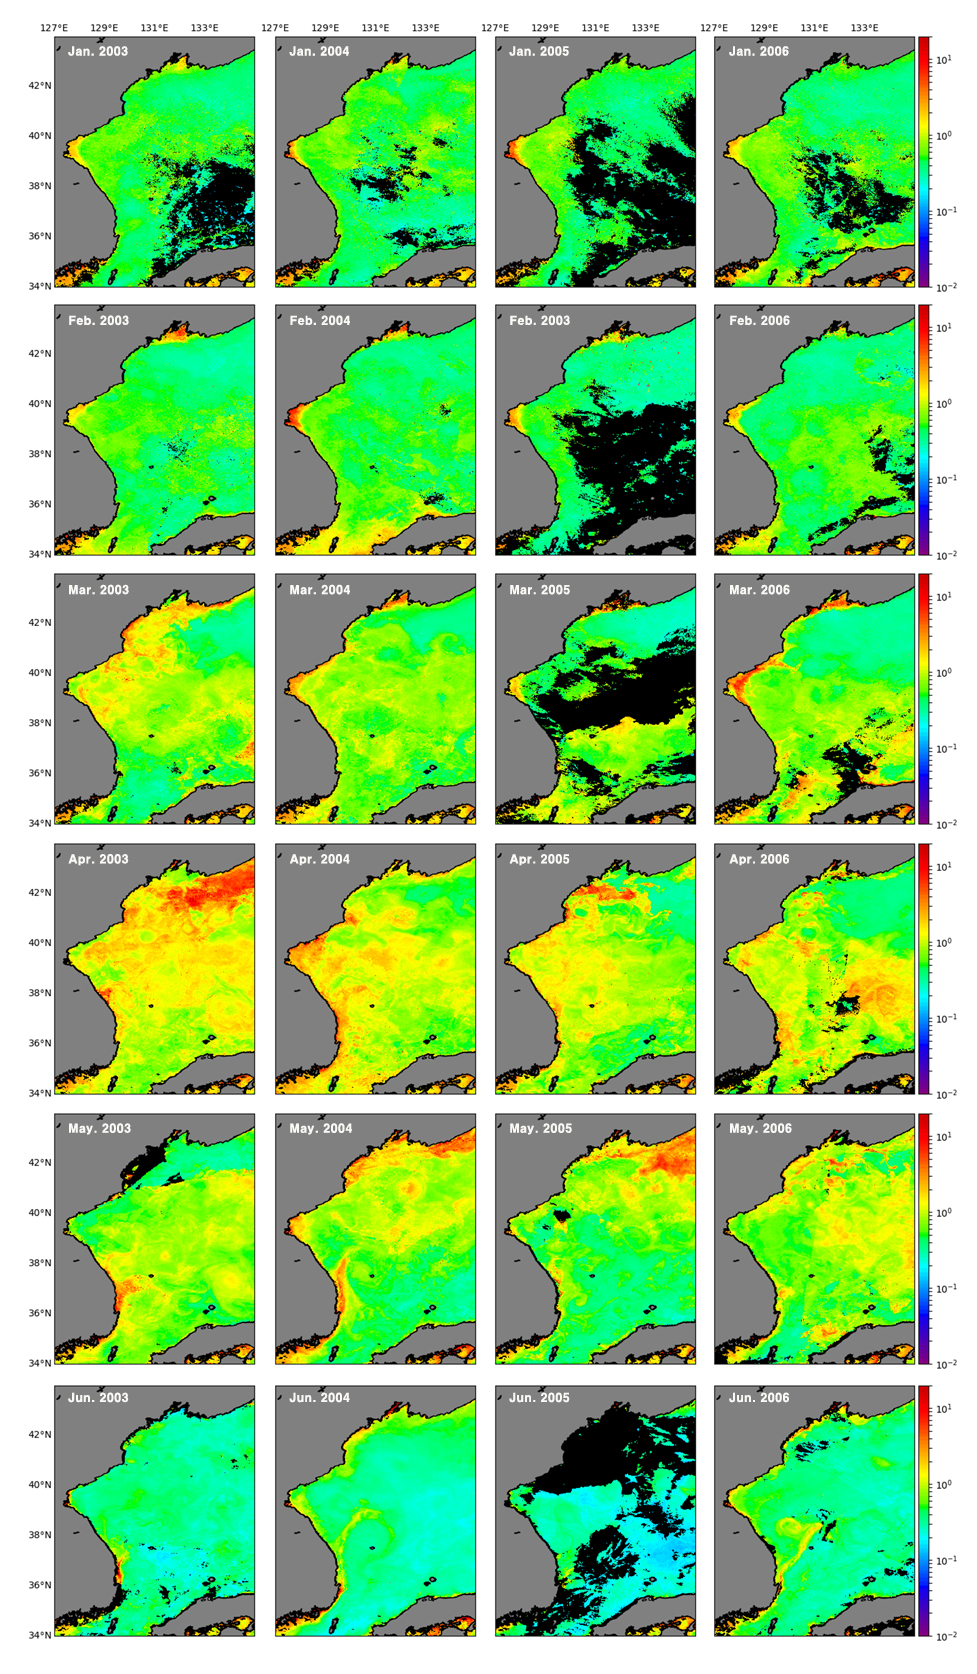
\includegraphics[width=0.8\linewidth]{../images/noname01}\\
	\caption{The monthly-mean chlorophyll-a distribution in the Korean East Sea, LAC. From 2003 to 2006, January to June. The unit of the color bar is $\rm mg/m^3$.}
	\label{fig:noname01}
\end{figure}
 

\begin{figure}
	\centering
	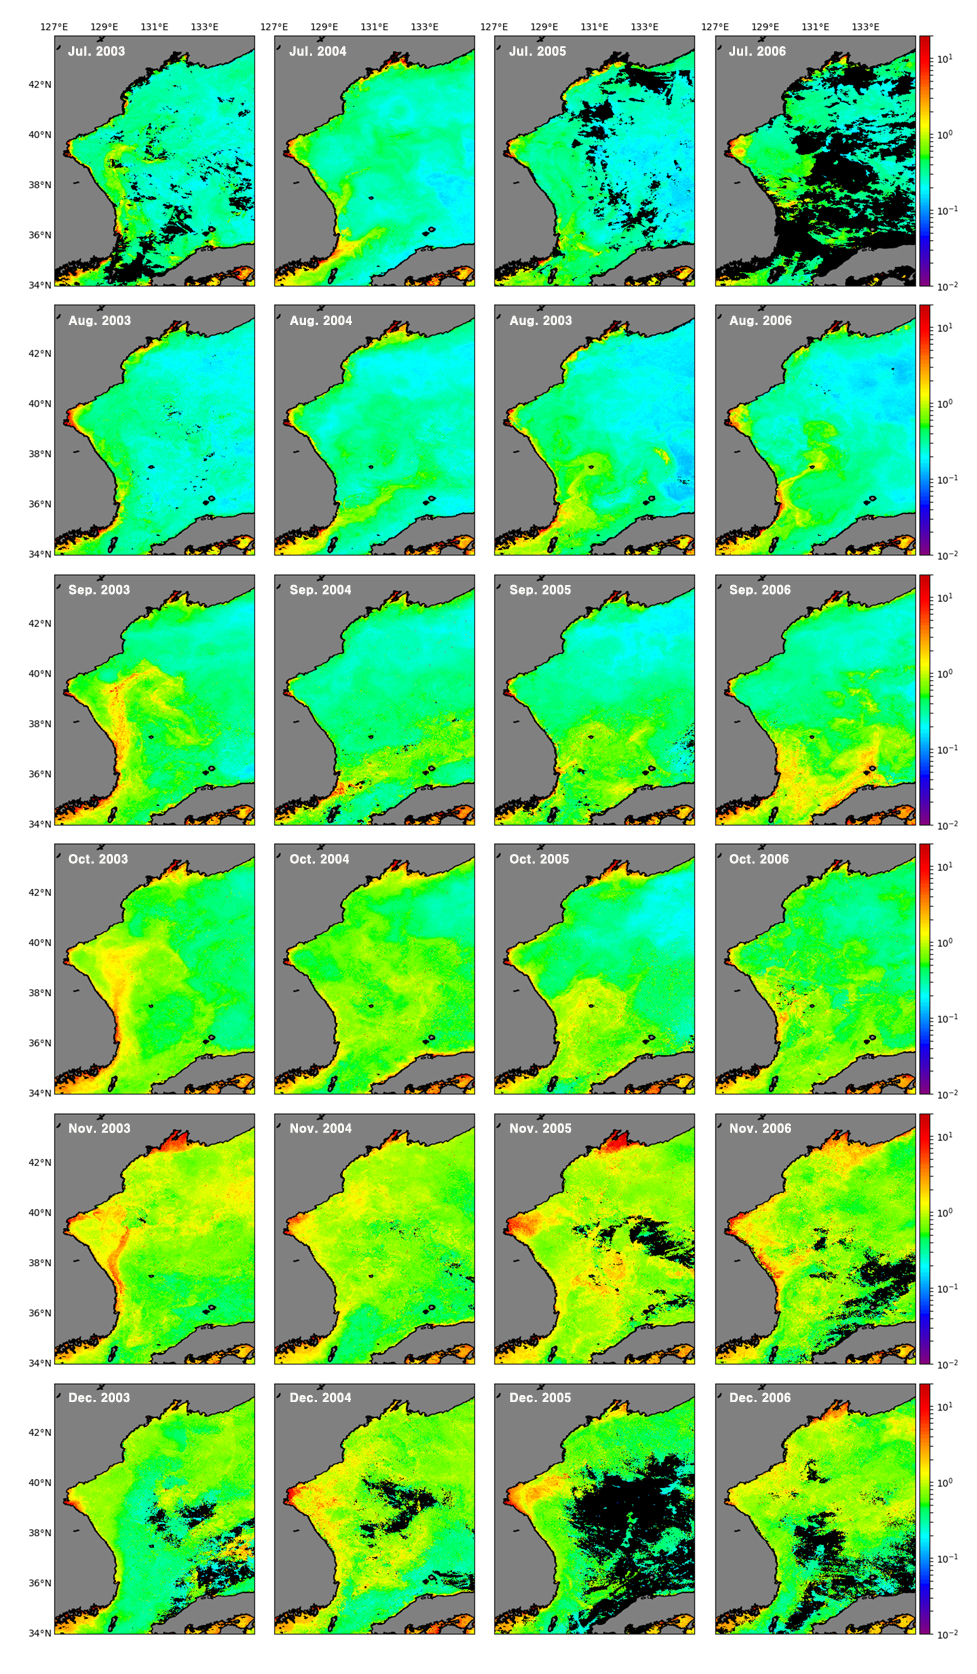
\includegraphics[width=0.8\linewidth]{../images/noname02}
	\caption{The monthly-mean chlorophyll-a distribution in the Korean East Sea, LAC. From 2003 to 2006, July to December. The unit of the color bar is $\rm mg/m^3$.}
	\label{fig:noname02}
\end{figure}

\begin{figure}
	\centering
	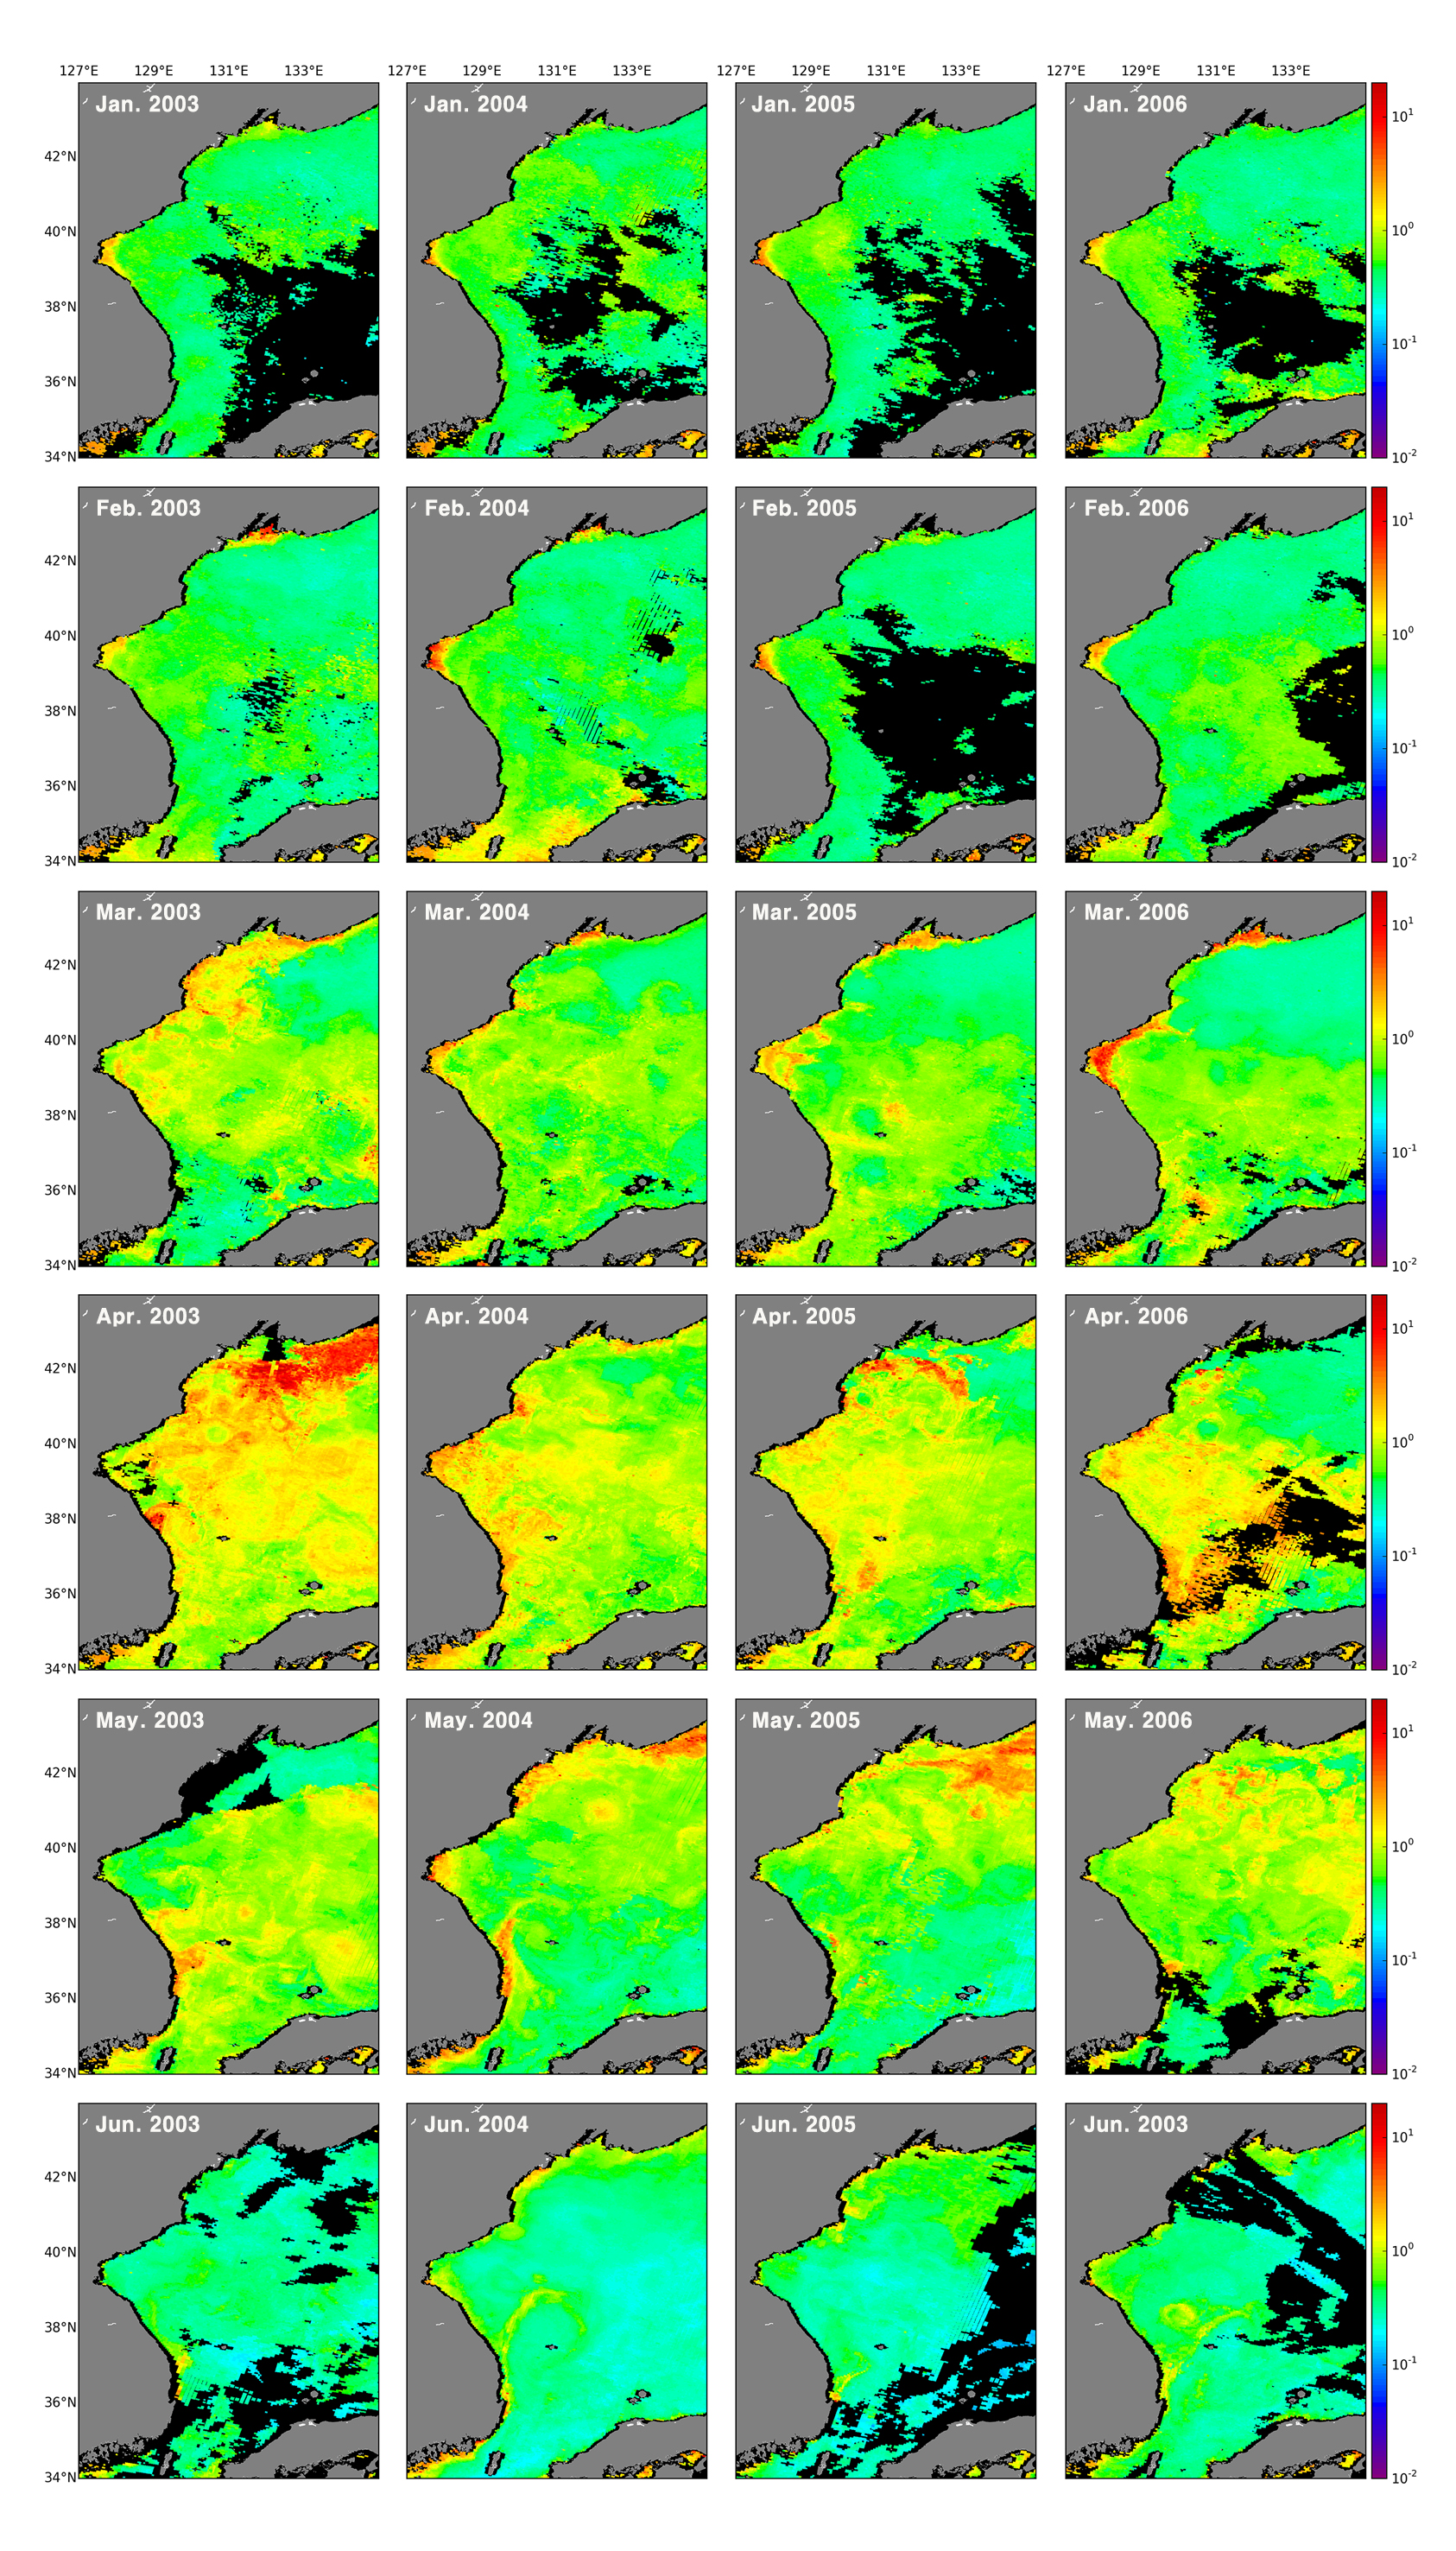
\includegraphics[width=0.8\linewidth]{../images/noname03}
	\caption{The monthly-mean chlorophyll-a distribution in the Korean East Sea, GAC. From 2003 to 2006, January to June. The unit of the color bar is $\rm mg/m^3$.}
	\label{fig:noname03}
\end{figure}

\begin{figure}
	\centering
	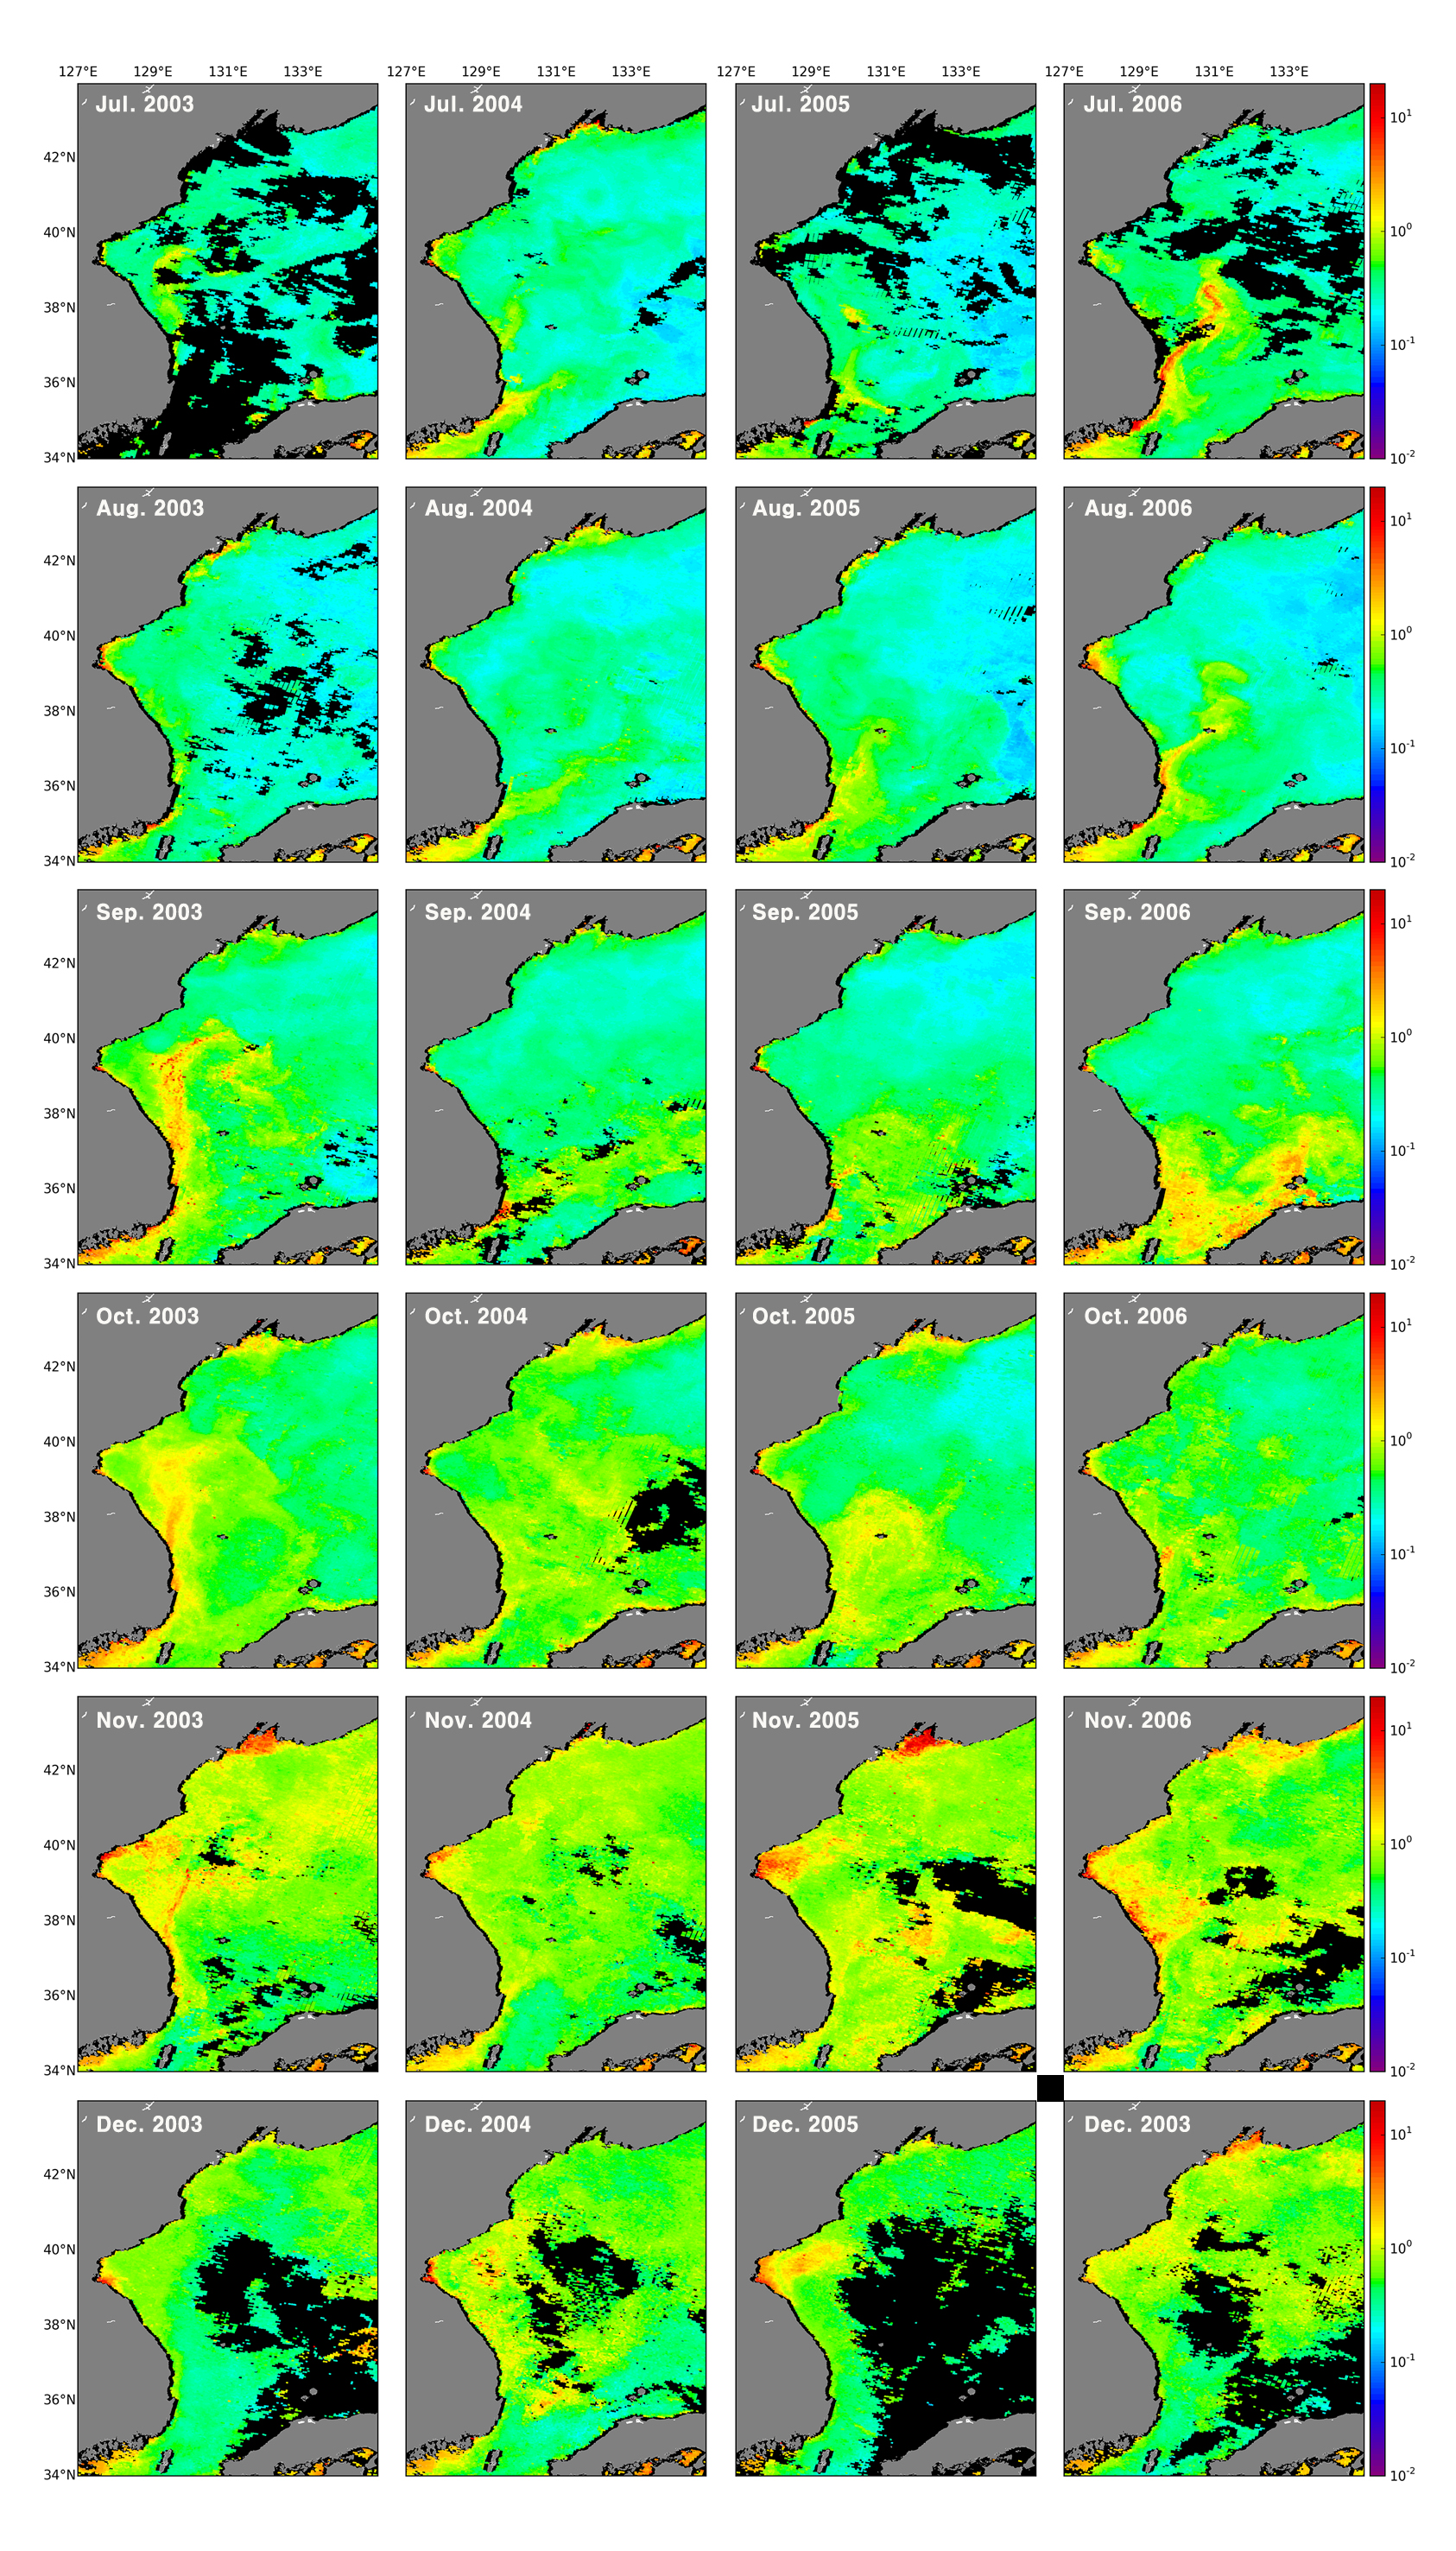
\includegraphics[width=0.8\linewidth]{../images/noname04}
	\caption{The monthly-mean chlorophyll-a distribution in the Korean East Sea, GAC. From 2003 to 2006, July to December. The unit of the color bar is $\rm mg/m^3$.}
	\label{fig:noname04}
\end{figure}
 
\subsection{The Effect of Spatial Resolution on the Data}
 
To find the effect of spatial resolution on the data, we compare the histograms of LAC data and the GAC data of April, 2003. We find that the histogram of GAC data shows more discontinuous shape compared to the LAC data in Figure.9. From the fact that a histogram of real data has continuous shape, it can be inferred that using LAC data is more accurate than using GAC data. The histogram of GAC data also shows more pixels with over 10 mg/m3 of chlorophyll-a concentration with sporadic distribution. These pixels are the speckles from previous researches (Chae, H. J., and Park, K., 2009; Hu, C., Carder, K. L., and Muller-Karger, F. E., 2001) also showing that LAC data is more appropriate for studying chlorophyll-a concentration.
  
  
  Figure 7 The monthly chlorophyll-a mean histogram in the Korean East Sea on April, 2003, (a) LAC (b) GAC.
  
  
   In Figure 10, part of the data with high chlorophyll-a concentration is enlarged to compare between LAC data and GAC data. LAC data has 6 pixels over 10 mg/m3, while GAC data has more than 100 pixels over 10 $\rm mg/m^3$. Such result occurs since one high-concentration value in GAC data affects a large area compared to LAC because of its low resolution.
  In Figure 11, part of the data with speckles is enlarged to compare between LAC data and GAC data. GAC data has a larger size of speckle because it has low resolution. In other words, it has more errors. Even if the speckles of the GAC data has been corrected, it will correct larger area compared to LAC causing a larger gap between the real value. In addition, even with the speckle correction applied using corrected LAC data will be more accurate.
  
  Figure 8. The monthly chlorophyll-a mean distribution in the Korean East Sea on April, 2003, (a) LAC (b) GAC. Enlarged an area with high concentrations of chlorophyll-a
  
  Figure 9. The monthly chlorophyll-a mean distribution in the Korean East Sea on April, 2003, (a) LAC (b) GAC. Enlarged an area with speckles
  
  
  
  

	
\section{Results}

\subsection{Calculation of the Monthly mean of Chlorophyll-a Concentration in the East Sea (Sea of Japan)}
The monthly-mean chlorophyll-a concentration of LAC from 2003 to 2006 is shown in Figure \ref{fig:monGAC01} - \ref{fig:monGAC03}. The monthly-mean chlorophyll-a concentration of GAC from 2003 to 2006 is shown in Figure \ref{fig:monGAC01} - \ref{fig:monGAC03}. The grey area is land showing Korea at the west and Japan at the southeast. Red means high concentration than the blue as it can be told from the color bar. Spring (March, April, May) and fall (October, November) show high concentration. The black area is part with no data due to cloud coverage or satellite failures. 

\begin{figure}[p]
	\centering
	\includegraphics[width=1.0\linewidth]{monLAC01}\\
	\caption{The monthly-mean chlorophyll-a distribution in the East Sea (Sea of Japan), LAC. From 2003 to 2006, January to April. The unit of the color bar is $\rm mg/m^3$.}
	\label{fig:monLAC01}
\end{figure}


\begin{figure}[p]
	\centering
	\includegraphics[width=1.00\linewidth]{../images/monLAC02}\\
	\caption{The monthly-mean chlorophyll-a distribution in the East Sea (Sea of Japan), LAC. From 2003 to 2006, May to August. The unit of the color bar is $\rm mg/m^3$.}
	\label{fig:monLAC02}
\end{figure}

\begin{figure}[p]
	\centering
	\includegraphics[width=1.00\linewidth]{../images/monLAC03}\\
	\caption{The monthly-mean chlorophyll-a distribution in the East Sea (Sea of Japan), LAC. From 2003 to 2006, September to December. The unit of the color bar is $\rm mg/m^3$.}
	\label{fig:monLAC03}
\end{figure}


\begin{figure}[p]
	\centering
	\includegraphics[width=1.0\linewidth]{../images/monGAC01}\\
	\caption{The monthly-mean chlorophyll-a distribution in the East Sea (Sea of Japan), LAC. From 2003 to 2006, January to April. The unit of the color bar is $\rm mg/m^3$.}
	\label{fig:monGAC01}
\end{figure}


\begin{figure}[p]
	\centering
	\includegraphics[width=1.00\linewidth]{../images/monGAC02}\\
	\caption{The monthly-mean chlorophyll-a distribution in the East Sea (Sea of Japan), LAC. From 2003 to 2006, May to August. The unit of the color bar is $\rm mg/m^3$.}
	\label{fig:monGAC02}
\end{figure}


\begin{figure}[p]
	\centering
	\includegraphics[width=1.00\linewidth]{../images/monGAC03}\\
	\caption{The monthly-mean chlorophyll-a distribution in the East Sea (Sea of Japan), LAC. From 2003 to 2006, September to December. The unit of the color bar is $\rm mg/m^3$.}
	\label{fig:monGAC03}
\end{figure}


\newpage
 
\subsection{The Annual Variability of Chlorophyll-a Concentration in the East Sea (Sea of Japan)}
 

%%%%%%%%%%%%%%%%%%%%%%%%%%%%%%%%%%%%%%%%%%%%%%%%%%%%%%%%%%%%%%%%%%%%%%%%%%   
% \begin{figure}[b]
% 	\centering
% 	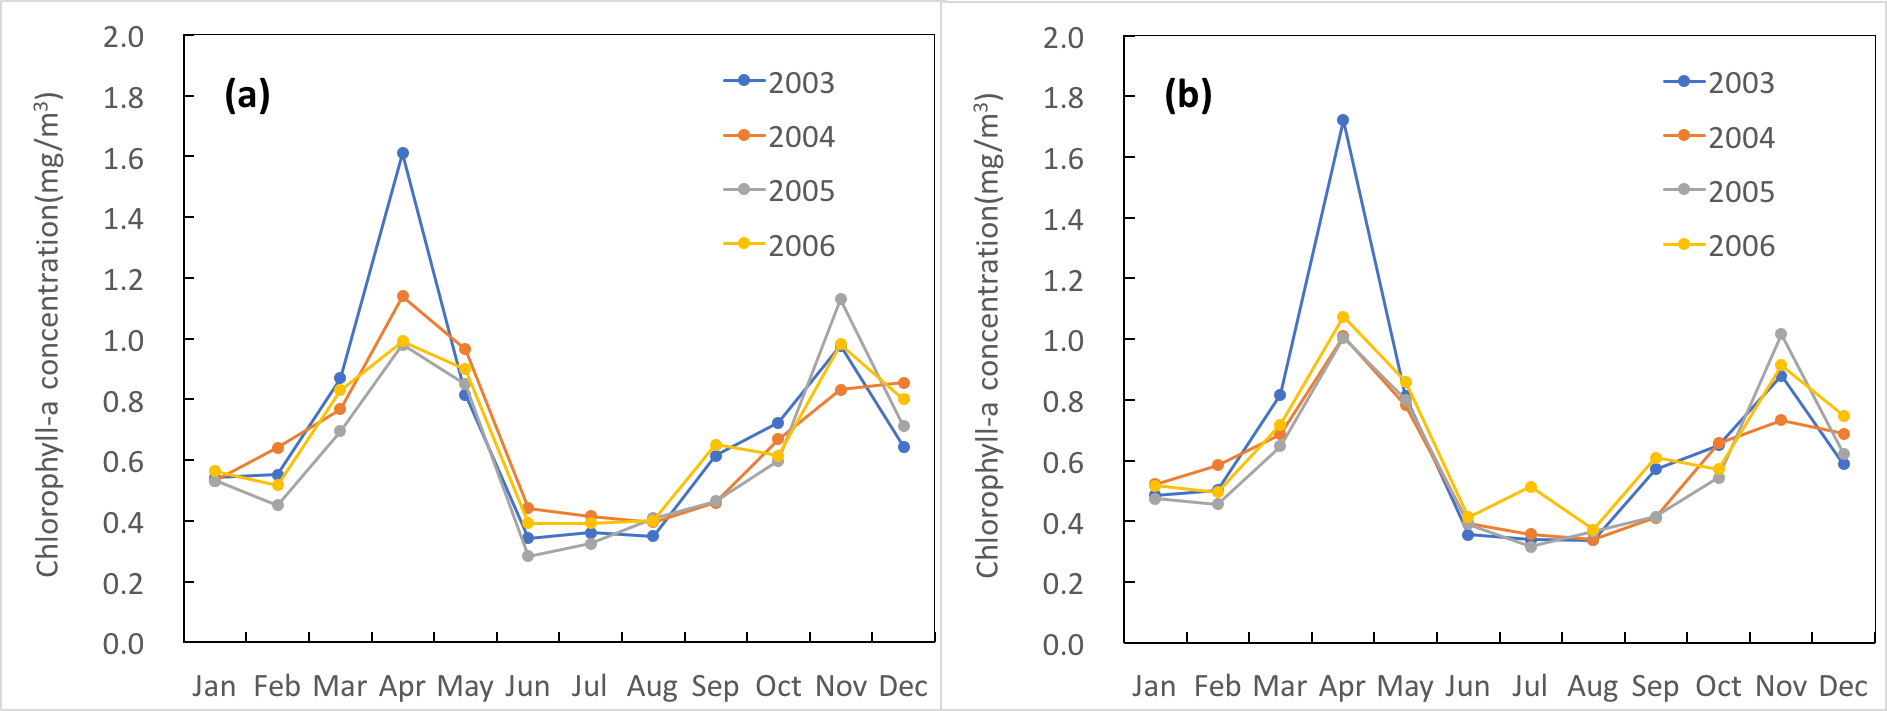
\includegraphics[width=1.0\linewidth]{../images/annualmon}\\
% 	\caption{The annual variability of monthly-mean chlorophyll-a concentration in the East Sea (Sea of Japan) from 2003 to 2006, (a) LAC (b) GAC.}
% 	\label{fig:annualmon}
% \end{figure}

%%%%%%%%%%%%%%%%%%%%%%%%%%%%%%%%%%%%%%%%%%%%%%%%%%%%%%%%%%%%%%%%%%%%%%%%%%   

 \begin{figure}[h]
	\begin{tikzpicture}
	\begin{axis} [
	width=1.0\linewidth,   height = 5cm, 
	major x tick style = transparent,
	xtick = data,
	%grid=major, 
	%zeichnet Koordinatengitter
	symbolic x coords={Jan, Feb, Mar, Apr, May, Jun, Jul, Aug, Sep, Oct, Nov, Dec},
	%	xlabel= Kraft $\lbrack{}$ \si{F} $\rbrack$, 
	%xmin=0, xstep=4, xmax=47,
	ylabel= chlorophyll-a concentration ($\rm mg/m^3$),
	ymin=0,	ystep=0.5, 	ymax=3.1,
	scaled y ticks = false,
	%nodes near coords, % data 값 표시
	% % % % % Ausrichten der Punktbeschriftung
	every node near coord/.append style={font=\scriptsize,/pgf/number format/precision=3}]
	\addplot table [x=Month, y=2003] {monLAC.csv}; \addlegendentry{2003}
	\addplot table [x=Month, y=2004] {monLAC.csv}; \addlegendentry{2004}
	\addplot table [x=Month, y=2005] {monLAC.csv}; \addlegendentry{2005}
	\addplot table [x=Month, y=2006] {monLAC.csv}; \addlegendentry{2006}
	%   \fill[gray,fill opacity=0.25] (axis cs:5,0) rectangle (axis cs:7,12); %Bereich einfügen
	\end{axis}
	\end{tikzpicture}
	
	\begin{tikzpicture}
	\begin{axis} [
	width=1.0\linewidth,   height = 5cm, 
	major x tick style = transparent,
	xtick = data,
	%grid=major, 
	%zeichnet Koordinatengitter
	    symbolic x coords={Jan, Feb, Mar, Apr, May, Jun, Jul, Aug, Sep, Oct, Nov, Dec},
	%	xlabel= Kraft $\lbrack{}$ \si{F} $\rbrack$, 
	%	xmin=0,
	%	xmax=15,
	ylabel= chlorophyll-a concentration ($\rm mg/m^3$),
	ymin=0,	ystep=0.5, 	ymax=3.1,
	%xmin=0, xstep=4, xmax=47,
	scaled y ticks = false,
	%nodes near coords, % data 값 표시
	% % % % % Ausrichten der Punktbeschriftung
	every node near coord/.append style={font=\scriptsize,/pgf/number format/precision=3},]
	[legend pos=north east]
	\addplot table [x=Month, y=2003] {monGAC.csv}; \addlegendentry{2003}
	\addplot table [x=Month, y=2004] {monGAC.csv}; \addlegendentry{2004}
	\addplot table [x=Month, y=2005] {monGAC.csv}; \addlegendentry{2005}
	\addplot table [x=Month, y=2006] {monGAC.csv}; \addlegendentry{2006}

	%   \fill[gray,fill opacity=0.25] (axis cs:5,0) rectangle (axis cs:7,12); %Bereich einfügen
	\end{axis}
	\end{tikzpicture}
 	\caption{The annual variability of monthly-mean chlorophyll-a concentration in the East Sea (Sea of Japan) from 2003 to 2006, (a) LAC (b) GAC.}
	\label{fig:annualmon}
\end{figure}

The annual variability of chlorophyll-a concentration in the East Sea (Sea of Japan) from 2003 - 2006 is shown in Figure 1, Figure 2. Both the LAC data and the GAC data has similar tendency, showing peaks on spring (April) and fall (November). The maximum/minimum value of LAC and GAC data was each 1.61 $\rm mg/m^3$ / 0.28 $\rm mg/m^3$, and 1.72 $\rm mg/m^3$ / 0.32 $\rm mg/m^3$. The difference between the two data was not ignorable. This infer that the effect of spatial resolution on the data has to be considered.
It is shown in Figure \ref{fig:annualmon} that the annual variability of monthly-mean chlorophyll-a concentration in the East Sea (Sea of Japan) from 2003 to 2006, (a) LAC (b) GAC.

 
 
%%%%%%%%%%%%%%%%%%%%%%%%%%%%%%%%%%%%%%%%%%%%%%%%%%%%%%%%%%%%%%%%%%%%%%%% 
% \begin{figure}[b]
%	\centering
%	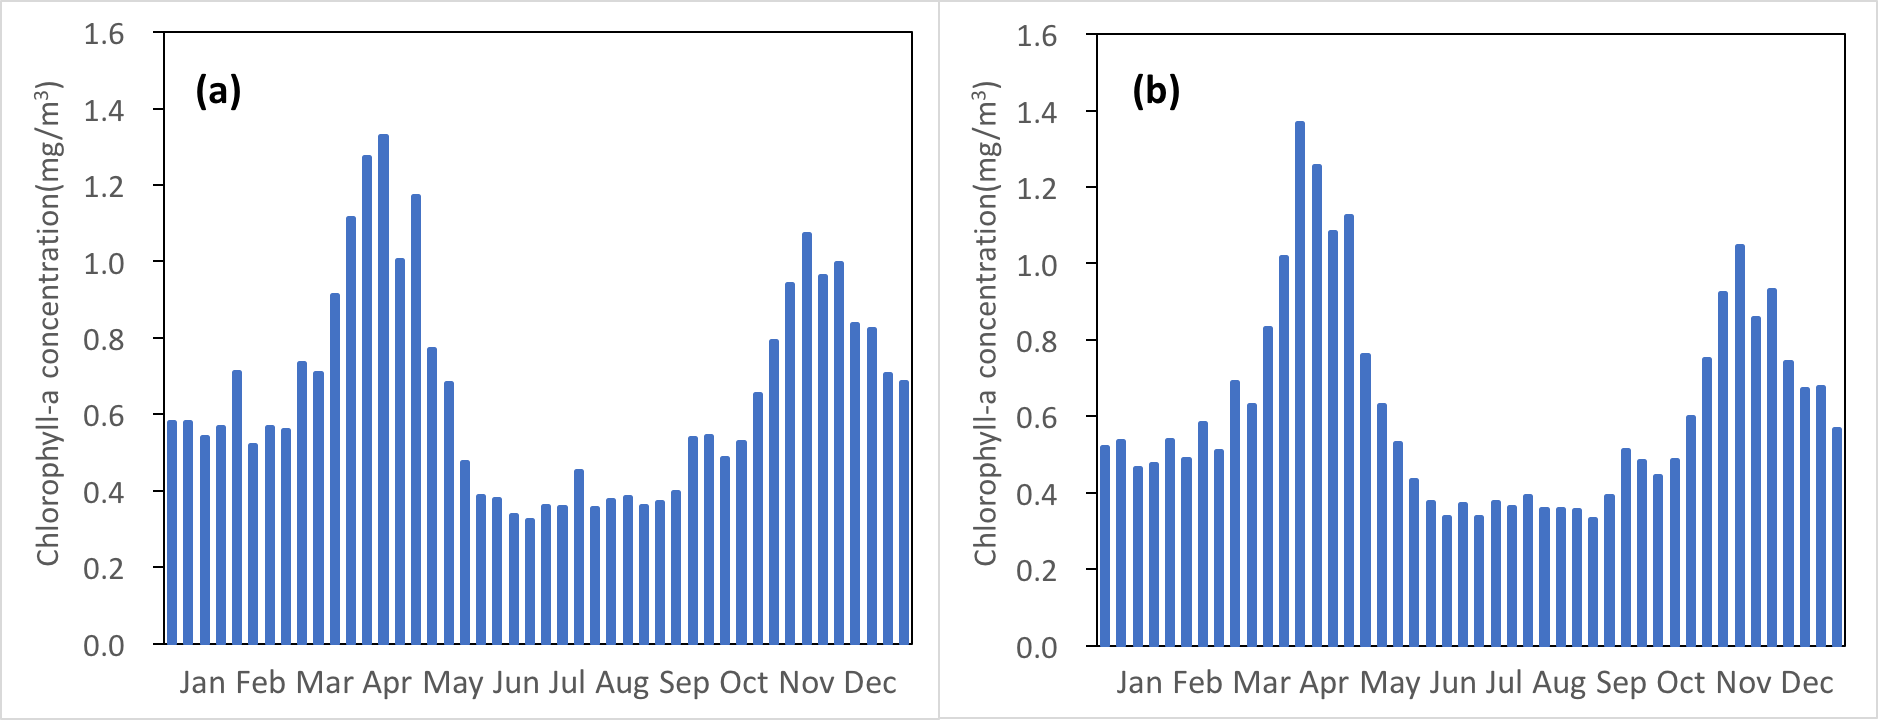
\includegraphics[width=1.0\linewidth]{../images/annualwky}\\
%	\caption{The annual variability of 8-day-mean chlorophyll-a concentration in the East Sea (Sea of Japan), (a) LAC (b) GAC. Each 8-day-mean data is average of data from 2003 to 2006.}
%	\label{fig:annuawkly}
%\end{figure}


  
  The annual variability of 8-day-mean chlorophyll-a concentration in the East Sea (Sea of Japan) from 2003 to 2006 is shown in Figure 3, Figure 4. This result allowed more concrete analysis of the data. The spring peak had 1.2 - 1.3 $\rm mg/m^3$ of chlorophyll-a concentration and was higher than the fall peak which had the value of 0.9 - 1.0 $\rm mg/m^3$. Winter had a higher concentration (0.6 $\rm mg/m^3$) compared to summer (0.4 $\rm mg/m^3$). The chlorophyll-a concentration in the East Sea (Sea of Japan) had clear seasonal differences. Both the LAC data and the GAC data was sufficient to show the seasonal differences. However, even though the 8-day-mean data was created using average of 4 years, the time of maximum concentration was different. 
  
  Part of the LAC data (2004 46th 8-day-mean, 2005 11th 8-day-mean, 2005 31th 8-day-mean) had been lost due to satellite failures. The data for these dates were substituted with the average of the adjacent data. This did not have a significant effect on the tendency, so the error was ignorable.
 
\begin{figure}[h]
	\begin{tikzpicture}
	\begin{axis} 
	[ width=0.98\linewidth,   height = 7cm, 
	major x tick style = transparent,
	xtick = data,
	%grid=major, 
	%zeichnet Koordinatengitter
	xmin=0, xstep=4, xmax=47,
	%symbolic x coords={5, 10, 15, 20, 25,30, 35, 40, 45, 50},
	%xlabel= Kraft $\lbrack{}$ \si{F} $\rbrack$, 
	ylabel= {\sffamily\small chlorophyll-a concentration ($\rm mg/m^3$)},
ymin=0,	ystep=0.5, 	ymax=3.1,
scaled y ticks = false,
%nodes near coords, % data 값 표시
% % % % % Ausrichten der Punktbeschriftung
every node near coord/.append style={font=\scriptsize,/pgf/number format/precision=3}]
[legend pos=north east]
\addplot table [x=Week, y=2003] {wkyLAC.csv}; \addlegendentry{\sffamily\scriptsize 2003}
\addplot table [x=Week, y=2004] {wkyLAC.csv}; \addlegendentry{\sffamily\scriptsize 2004}
\addplot table [x=Week, y=2005] {wkyLAC.csv}; \addlegendentry{\sffamily\scriptsize 2005}
\addplot table [x=Week, y=2006] {wkyLAC.csv}; \addlegendentry{\sffamily\scriptsize 2006}
%   \fill[gray,fill opacity=0.25] (axis cs:5,0) rectangle (axis cs:7,12); %Bereich einfügen
\end{axis}
\end{tikzpicture}

\begin{tikzpicture}
\begin{axis} 
[ width=0.98\linewidth,   height = 7cm, 
major x tick style = transparent,
xtick = data,
%grid=major, 
%zeichnet Koordinatengitter
xmin=0, xstep=4, xmax=47,
%symbolic x coords={Jan, Feb, Mar, Apr, May, Jun, Jul, Aug, Sep, Oct, Nov, Dec},
%xlabel= Kraft $\lbrack{}$ \si{F} $\rbrack$, 
ylabel= {\sffamily\small chlorophyll-a concentration ($\rm mg/m^3$)},
ymin=0,	ystep=0.5, 	ymax=3.1,
scaled y ticks = false,
%nodes near coords, % data 값 표시
% % % % % Ausrichten der Punktbeschriftung
every node near coord/.append style={font=\scriptsize,/pgf/number format/precision=3}]
[legend pos=north east]
\addplot table [x=Week, y=2003] {wkyGAC.csv}; \addlegendentry{\sffamily\scriptsize 2003}
\addplot table [x=Week, y=2004] {wkyGAC.csv}; \addlegendentry{\sffamily\scriptsize 2004}
\addplot table [x=Week, y=2005] {wkyGAC.csv}; \addlegendentry{\sffamily\scriptsize 2005}
\addplot table [x=Week, y=2006] {wkyGAC.csv}; \addlegendentry{\sffamily\scriptsize 2006}
%   \fill[gray,fill opacity=0.25] (axis cs:5,0) rectangle (axis cs:7,12); %Bereich einfügen

\end{axis}
\end{tikzpicture}
\caption{The annual variability of 8-day-mean chlorophyll-a concentration in the East Sea (Sea of Japan), (a) LAC (b) GAC. Each 8-day-mean data is average of data from 2003 to 2006.}
\label{fig:annuawkly}
\end{figure}



\subsection{The Effect of Spatial Resolution on the Data}
 
To find the effect of spatial resolution on the data, we compare the histograms of LAC data and the GAC data of April, 2003. We find that the histogram of GAC data shows more discontinuous shape compared to the LAC data in Figure \ref{fig:monHIS}. From the fact that a histogram of real data has continuous shape, it can be inferred that using LAC data is more accurate than using GAC data. The histogram of GAC data also shows more pixels with over $\rm mg/m^3$ of chlorophyll-a concentration with sporadic distribution. These pixels are the speckles from previous researches (Chae, H. J., and Park, K., 2009; Hu, C., Carder, K. L., and Muller-Karger, F. E., 2001) also showing that LAC data is more appropriate for studying chlorophyll-a concentration \cite{chae2009characteristics,hu2001precise}.
  
\begin{figure}[h]
	\centering
	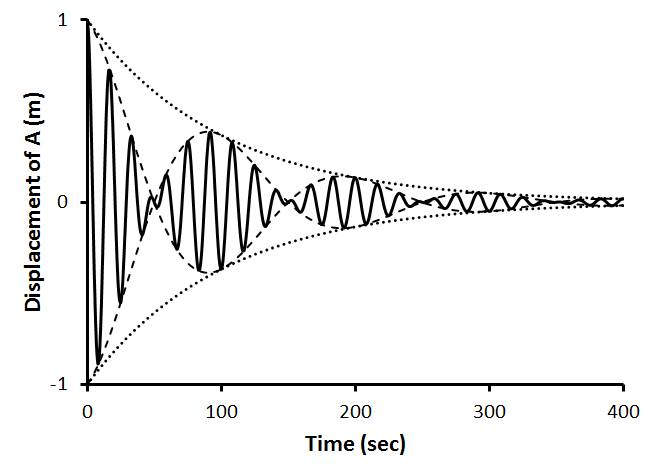
\includegraphics[width=0.8\linewidth]{../images/monHIS}\\
	\caption{The monthly chlorophyll-a mean histogram in the East Sea (Sea of Japan) on April, 2003, (a) LAC (b) GAC.}
	\label{fig:monHIS}
\end{figure}
 
In Figure\ref{fig:monHISHI}, part of the data with high chlorophyll-a concentration is enlarged to compare between LAC data and GAC data. LAC data has 6 pixels over $\rm mg/m^3$, while GAC data has more than 100 pixels over 10 $\rm mg/m^3$. Such result occurs since one high-concentration value in GAC data affects a large area compared to LAC because of its low resolution.
In Figure\ref{fig:monHISSPEC}, part of the data with speckles is enlarged to compare between LAC data and GAC data. GAC data has a larger size of speckle because it has low resolution. In other words, it has more errors. Even if the speckles of the GAC data has been corrected, it will correct larger area compared to LAC causing a larger gap between the real value. In addition, even with the speckle correction applied using corrected LAC data will be more accurate.
    
  \begin{figure}[h]
  	\centering
  	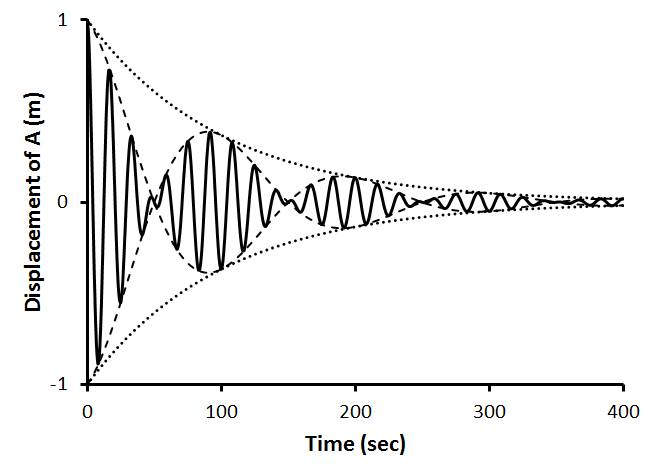
\includegraphics[width=0.8\linewidth]{../images/monHISHI}\\
  	\caption{The monthly chlorophyll-a mean distribution in the East Sea (Sea of Japan) on April, 2003, (a) LAC (b) GAC. Enlarged an area with high concentrations of chlorophyll-a.}
  	\label{fig:monHISHI}
  \end{figure}
  
    \begin{figure}[h]
  	\centering
  	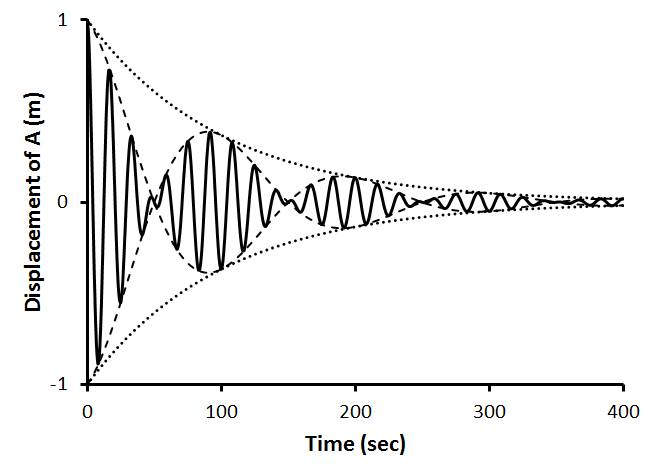
\includegraphics[width=0.8\linewidth]{../images/monHISSPEC}\\
  	\caption{The monthly chlorophyll-a mean distribution in the East Sea (Sea of Japan) on April, 2003, (a) LAC (b) GAC. Enlarged an area with speckles.}
  	\label{fig:monHISSPEC}
  \end{figure}
  
%	
\section{test}

	\begin{figure} [b]
	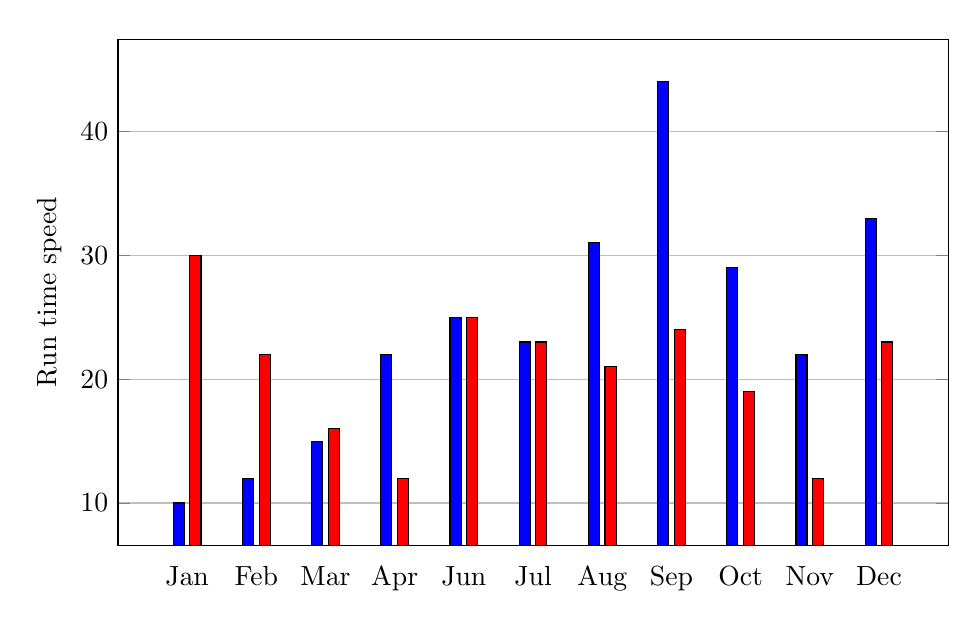
\begin{tikzpicture}	
	\begin{axis} [
	width=1.0\linewidth,      height = 8cm, 
     major x tick style = transparent,
      xtick = data,
	ybar,
	bar width=4pt,
	ymajorgrids = true,
    ylabel = {Run time speed},
       scaled y ticks = false,
    symbolic x coords={Jan, Feb, Mar, Apr, Jun, Jul, Aug, Sep, Oct, Nov, Dec},
	]
	\addplot[ybar,fill=blue] coordinates { (Jan, 10) (Feb, 12) (Mar,15) (Apr,22) (Jun,25) (Jul,23) (Aug,31) (Sep,44) (Oct,29) (Nov,22) (Dec,33) };
	\addplot[ybar,fill=red] coordinates { (Jan, 30) (Feb, 22) (Mar,16) (Apr,12) (Jun,25) (Jul,23) (Aug,21) (Sep,24) (Oct,19) (Nov,12) (Dec,23) };
	\end{axis}
	\end{tikzpicture}
	\caption{Chart name.}
	\label{fig:annu}
	\end{figure}
	figure \ref{fig:annu}.
	
	
	\begin{figure} 
 \begin{tikzpicture}
	\begin{axis} [
		width=1\linewidth,   height = 8cm, 
	major x tick style = transparent,
	    xtick = data,
	%grid=major, 
	%zeichnet Koordinatengitter
    symbolic x coords={Jan, Feb, Mar, Apr, May, Jun, Jul, Aug, Sep, Oct, Nov, Dec},
%	xlabel= Kraft $\lbrack{}$ \si{F} $\rbrack$, 
%	xmin=0,
%	xmax=15,
	ylabel= Strom $\lbrack{}$ \si{kA} $\rbrack$,
	ymin=0,
	ystep=.25
	ymax=2.0,
	scaled y ticks = false,
	%nodes near coords, % data 값 표시
	% % % % % Ausrichten der Punktbeschriftung
	every node near coord/.append style={font=\scriptsize,/pgf/number format/precision=3}]
	\addplot table [x=Month, y=2003] {momGAC.csv};
	\addplot table [x=Month, y=2004] {momGAC.csv};
	\addplot table [x=Month, y=2005] {momGAC.csv};
	\addplot table [x=Month, y=2006] {momGAC.csv};

%   \fill[gray,fill opacity=0.25] (axis cs:5,0) rectangle (axis cs:7,12); %Bereich einfügen

	\end{axis}
	\end{tikzpicture}

		\caption{Chart name.}
		\label{fig:annu}
	\end{figure}
	figure \ref{fig:annu}.
	

	

	% Next Section (e.g. Experiment, Linear theory, etc...) 
	% 이외에도 추가로 section마다 파일을 sub 폴더 안에 넣고 여기에서 
	% include 해주면 됩니다.
	% 예시 : methodology.tex을 sub 폴더안에 저장, 이 자리에 
	% \section{Methodology}

\subsection{Study area}

<<<<<<< HEAD
The East Sea (Sea of Japan) was chosen to calculate chlorophyll-a concentration using the ocean color data. The study area is shown in Figure \ref{fig:Map_of_Research_Area}. as 34.00°N - 44.00°N, 127.°E - 135.00°E which covers the whole East Sea (Sea of Japan) near Korea. The South Sea and the Yellow Sea was excluded from the study area because it is difficult to calculate the chlorophyll-a concentration using the ocean color algorithm due to their shallow depth. 

The depth of the East Sea rapidly increases from the east coast. The East has a surface area of about 978,000 $\rm km^2$, a mean depth of 1,752 $\rm m $ and a maximum depth of 3,742 $\rm m$. Such depth allows to use the developed chlorophyll-a algorithms. Terrains under the East Sea near Korean Peninsula is complex and the area of the continental shelf is steep.

\begin{figure}[h]

	\centering
{\includegraphics[width=0.95\textwidth]	{Map_of_Research_Area} }

\caption{Map showing study area.}
	\label{fig:Map_of_Research_Area}

\end{figure}

\newpage


\subsection{SeaWiFS data and Study period}

SeaWiFS ocean color data is used in order to calculate chlorophyll-a concentration of the East Sea (Sea of Japan) in this study. However, it is not able to obtain recent measurements since SeaWiFS had only activated from September 1997 to December 2010. {Table \ref{table01}.} shows the mission charactoristics of SeaWiFS and Table \ref{table02} shows the Cahracteristics of the SeaWiFS ocean color sensor \cite{hooker1992An}.

 \begin{table}[h]%[width=1.0\linewidth]
 	\caption{The mission characteristics of SeaWiFS.}
 	\label{table01}
 	\centering
 	\begin{tabular}{c|c}
 		\hline \setlength{\arrayrulewidth}{0.8pt}. 
 	Orbit Type	& Sun Synchronous at 705 km \\ \hline
 	Equator Crossing &	Noon +20 min, descending \\ \hline
 	Orbital Period &	99 minutes  \\ \hline
 	Swath Width &	2,801 km LAC/HRPT (58.3 degrees)  \\ \hline
 	Swath Width &	1,502 km GAC (45 degrees)  \\ \hline
 	Spatial Resolution &	1.1 km LAC, 4.5 km GAC  \\ \hline
 	Real-Time Data Rate &	665 kbps  \\ \hline
 	Revisit Time &	1 day  \\ \hline
 	Digitization &	10 bits  \\ \hline
 	\end{tabular}
 \end{table}

 \begin{table}[h]%[width=1.0\linewidth]
	\caption{Cahracteristics of the DeaWiFS ocean color sensor.}
	\label{table02}
	\centering
	\begin{tabular}{c|c|c|c|c}
		\hline \setlength{\arrayrulewidth}{0.8pt}. 
		Band	& Wavelength FWHM[nm] & Saturation Radiance & Input Radiance & SNR\\ \hline{5.0pt}
		1 & 402-422 & 13.63 & 9.10 & 499 \\ \hline
		2 & 433-453 & 13.25 & 8.41 & 674  \\ \hline
		3 & 480-500 & 10.50 & 6.56 & 667 \\ \hline
		4 & 500-520 & 9.08 & 5.64 & 640  \\ \hline
		5 & 545-565 & 7.44 & 4.57 & 596 \\ \hline
		6 & 660-680 & 4.20 & 2.46 & 442  \\ \hline
		7 & 745-785 & 3.00 & 1.61 & 455 \\ \hline
		8 & 845-885 & 2.13 & 1.09 & 467  \\ \hline
	\end{tabular}
\end{table}
 
 The Ocean Biology Processing Group collects and processes data from Earth-viewing satellites. These data are organized in various ways reflecting different spatial, temporal, and parameter groupings. Over the years, certain terminology about remote sensing data has arisen to describe these organizational conventions. Level-0 is unprocessed data from remote sensing instruments at a full resolution. Level-1 data is obtained through radiometric and geometric calibration. Level-2 data is made of geophysical variables processed from level-1 data using developed algorithms \cite{feldman2017ocean}. In this research, chlorophyll-a concentration is the geophyscial variable we choose to process.


The SeaWiFS Level-2 Ocean Color chlorophyll-a Data Version 2014 can be downloaded from the NASA Goddard Space Flight Center (GSFC) Distributed Active Archive Center (DAAC). Processing Level-1 data to Level-2 data was conducted by NASA, using NASA SeaDAS program\cite{NASASeaFiWSdata}. NASA SeaDAS uses two algorithms to create chlorophyll-a concentration data from the Level-1 data of remote sensing reflectance ($\rm R_{rs}$); these algorithms are the OCx band ratio algorithm and the color index (CI) algorithm of Hu. 
 The OCx band ratio algorithm use the ratio of two bands in a fourth-order polynomial equation in a relation with chlorophyll-a. It can be expressed as \eqref{eq:001}.
 
 \begin{equation}
 {\rm log_{10} (chlor_a) = a_0 + \sum_{i=1}^4 a_i ~ log_{10} \left( \frac{(R_{rs}(\lambda_{blue})}{(R_{rs}(\lambda_{green})} \right) ^i }
 \label{eq:001}
 \end{equation}
 
The coefficients $\rm a_0$ - $\rm a_4$ are values for each sensor acquired experimentally. The OCx algorithm was proved to be accurate by O’Reilly et. al\cite{o2000ocean}. The CI algorithm uses three bands and can be expressed as \eqref{eq:002}.

 \begin{equation}
{\rm CI = R_rs ({\lambda}_{green}) - [R_rs ({\lambda}_{blue}) + \frac {({\lambda}_{green}) - {\lambda}_{blue})} {({\lambda}_{red}) - {\lambda}_{blue}} * ({\lambda}_{red}) - R_rs ({\lambda}_{blue}) ]}
\label{eq:002}
\end{equation}

The $\rm {\lambda}_{blue}$, $\rm {\lambda}_{green}$, $\rm {\lambda}_{red}$ are wavelengths closest to 443 $\rm nm$, 555 $\rm nm$ and 670 $\rm nm$, different for each sensor. According to Hu, C., Lee, Z., and Franz, B., for the lower concentration of chlorophyll-a (less than 0.25 $\rm mg/m^3$), it is more accurate to use CI algorithm \cite{hu2012chlorophyll}. The NASA SeaDAS software uses CI algorithm for chlorophyll retrievals below 0.15 $\rm mg/m^3$, and OCx band ratio algorithm for retrievals above 0.2 $\rm mg/m^3$. For the concentration between 0.15 $\rm mg/m^3$ and 0.2 $\rm mg/m^3$, it blends both algorithm.

The level-2 GAC data of the East sea (Sea of Japan) can be obtained from 1997 to 2010 but the level-2 LAC data can be obtained only from 2003 to 2006. Only a few LAC data files of the East Sea (Sea of Japan) are available after 2007. That is why the study period was set from 2003 to 2006. The information of on used data is shown in Table \ref{data_information}.
The level-3 LAC and GAC data are derived geophysical variables that have been aggregated onto a well-defined over a well-defined time period and projected onto a well-defined spatial grid.

start 박기현 추가
 \begin{table}[h]
	\caption{The number of Level-2 files for analysis.}
	\label{data_information}
	\centering
	\begin{tabular}{c | c | c }
		\hline \setlength{\arrayrulewidth}{3.5pt}. 
			& LAC  & GAC \\ \hline
		2003 (N) & 482 & 490 \\ \hline
		2004 (N) & 441 & 497 \\ \hline
		2005 (N) & 270 & 494 \\ \hline
		2006 (N) & 313 & 498 \\ \hline
		total (N) & 1,506 & 1,979 \\ \hline
	\end{tabular}
\end{table}
end 박기현추가

\hfill \break
\hfill \break


 \subsection{Deriving Chlorophyll-a Concentration using LAC data and GAC data}
 
NASA SeaDAS is used to process the level-2 data of chlorophyll-a to level-3 data of monthly-mean/ 8-day-mean of chlorophyll-a concentration data. Monthly-mean data is created to show the overall tendency, while 8-day-mean data is created to see more specific tendency. Simple average method had been used to create the mean files. This method sums pixel values of chlorophyll-a at the same location and divides it by the number of data that have been compiled. This process also gives latitude longitude value to the pixels, creating a Standard Mapped Image (SMI). Chae, H. J., \& Park, K. (2009) used weighted average method to process data. However, according to Park, K. A., Park, J. E., Lee, M. S., \& Kang, C. K. (2012), both the weighted average method and the simple average method are suitable for processing SeaWiFS data in the East Sea (Sea of Japan). In addition, the more general method, the simple average method is used in this research.
  
 Since running each process using SeaDAS is inconvenient, so the process is automated by using python batch processing. This commands SeaDAS to repeat the process. Python can also create png files from the SMI. We use the obtained monthly-mean and 8-day-mean data to find the annual variability of chlorophyll-a concentration.
 
 The effect of spatial resolution on the data was studied by comparing the LAC and the GAC data. The monthly average data was compared and the differences of the values were calculated. Further analysis was done on pixels with a value over 10 $\rm mg/m^3$. The maximun value of each month was also compared. These research were done to find out which data showed more accuracy and precision
 
  와 같이 작성
	%%%% 주의
	%%%% 파일이 나뉠 때마다 자동으로 페이지넘김(\clearpage)가 됩니다. 
	%%%% 따라서 subsection을 나누는 용도로는 사용하지 마십시오.
	%%%% \include{sub/experiment} 와 같이...


	\section{Discussion}
Spring(April) and fall(November) each had 1.2 - 1.3 $\rm mg/m^3$, 0.9 - 1.0 $\rm mg/m^3$ of chlorophyll-a concentrations which was higher than the other seasons showing similarities with the result of Yamada, K., Ishizaka, J., Yoo, S., Kim, H. C. and Chiba, S. \cite{yamada2004seasonal}. Analysis of annual variability with the temporal resolution increased to 8-day-mean data showed winter (December, January, February) had higher concentration compared to summer (June, July, August), each with the values of 0.6 $\rm mg/m^3$ and $\rm mg/m^3$. This conclude that the Korean East Sea shows clear seasonal differences.

In a perspective of spatial resolution, both the LAC data and the GAC data were suitable for research on the chlorophyll-a concentration variability in the Korean East Sea. However, histogram analysis showed that GAC data had more speckles compared to LAC data. The pixel analysis of chlorophyll-a concentration data on April, 2003 also showed that even with the speckle correction it is more accurate to use LAC data because of its high resolution.

The limit of this research is that speckle errors were not corrected causing the concentration values to be higher than the in-situ data. Moreover, the in-situ data of the area of interest was not measured in this research so it could not directly show whether the LAC data or the GAC data is more accurate. Further research will compare the processed data of LAC and GAC with the in-situ data from previous researches.
 % Conclusion
	
	%%\clearpage  %%% Appendix를 새 페이지에서 시작
\appendix
\renewcommand{\thesection}{\Alph{section}} %%% TOC에 appendix numbering 재설정
\renewcommand{\thesubsection}{\arabic{subsection}}
\renewcommand{\thesubsubsection}{\arabic{subsubsection}}
\titleformat{\section}[hang] {\normalfont\fontsize{21}{21}\selectfont\bfseries}{\Alph{section}.}{1em}{} %%% Appendix section title의 재설정
\titleformat{\subsection}[hang] {\normalfont\fontsize{16}{16}\selectfont\bfseries}{\Alph{section}.\arabic{subsection}.}{1em}{}
\titleformat{\subsubsection}[hang] {\normalfont\fontsize{14}{14}\selectfont}{\Alph{section}.\arabic{subsection}.\arabic{subsubsection}.}{1em}{}
\titleformat{\paragraph}[hang] {\normalfont\fontsize{12}{12}\selectfont\it}{}{1em}{}
\renewcommand{\theequation}{\thesection.\arabic{equation}} %%% Appendix equation numbering 의 재설정
\renewcommand{\thefigure}{\thesection-\arabic{figure}} %%% Appendix figure numbering 의 재설정
\renewcommand{\thetable}{\thesection-\arabic{table}} %%% Appendix table numbering 의 재설정
\setcounter{equation}{0} %%% Appendix equation starting number의 초기화
\setcounter{figure}{0} %%% Appendix figure starting number의 초기화
\setcounter{table}{0} %%% Appendix table starting number의 초기화
\section{Appendix title}
논문의 구조 상 본문에 넣지는 못했지만 논문에 수록하고 싶은 부록(appendix)이 있다면 여기에 작성한다. Appendix는 반드시 있어야 하는 건 아니다. 만약 본문에서 연구 내용을 충분히 작성했다면 이 Appendix 파트 전체를 제거한다.  % Appendix가 없는 경우 주석처리하십시오
	
	\bibliography{bibfile} % 참고문헌
	% BibTeX 코드 쉽게 얻어오는 방법 %
	% Google Scholar 에서 검색한 결과에서 `인용'을 클릭한다.
	% BibTeX 코드를 얻고자 한다면, 하단의 `BibTeX' 을 클릭.
	% 코드가 나온다. Ctrl+A, Ctrl+C로 복사, bibfile에 붙여넣기.
	
	%\begin{summary}
\addcontentsline{toc}{section}{Summary}  %%% TOC에 표시
한글로 졸업논문을 작성한 학생은 반드시 5페이지 내외의 영어 요약문을 작성해야 합니다. 영문으로 작성하는 학생은 이 부분을 작성하지 않아도 됩니다.
\end{summary} % Summary
	%(영어로 작성한 학생은 이 부분을 주석 처리하십시오.)
	
	%-----------------------------------------------------
%   감사의 글
%-----------------------------------------------------
\begin{acknowledgements}
\addcontentsline{toc}{section}{Acknowledgements}  %%% TOC에 표시

%$# 아래 내용 골자로 해서 살을 붙이고, 에피소드 넣어서 작성하도록

%$# 이 논문은 미국 미시시피 주립대학에서 진행되었던 Overseas Research and education Program(ORP)의 지원을 받아 시작할 수 있었습니다. ORP를 담당했던 미시시피 주립대학의 Dr. Dash 교수님께 다시한번 감사드리며, Python coding, Ocean color data order, batch processing 등을 지도해 준 Madhur Dacoda에게도 감사드립니다.
 I would first like to thank Gyeonggi Science High school for the gifted for allowing us to study remote sensing through the Overseas Research and education Program(ORP) in Mississippi State University. Thanks for Dr. Padmanava Dash and Madhur Dacoda for teaching us about ocean color data with python coding and batch processing. The basic concepts and the methods that you have though us was really useful to process the data. The ORP program was more helpful with the support of Youngwoo Cho in Mississippi State University and my friend Jong Min, Choi and our teacher Kiehyun Park. The hardships we overcame while learning python was really meaningful.
 
 Lastly, I would like to thank Prof. Kyung Ae Park and Prof. Hak-sung Kim for revising this thesis. The overall comments and the specific corrections helped me to create a more professional thesis.  
%$# ORP 동안 도움을 주신 미시시피 주립대학의 Youngwoo Cho 선생님과 함께 참여한 경기과학고등학교의 친구 Jong Min, Choi, Kiehyun Park 선생님께도 감사를 드립니다.

%$# ORP 동안 도움을 주신 미시시피 주립대학의 Youngwoo Cho 선생님과 함께 참여한 경기과학고등학교의 친구 Jong Min, Choi, Kiehyun Park 선생님께도 감사를 드립니다. 감

%$# 경기과학고에 입학하여 무사히 졸업논문을 통과할 수 있도록 도와주신 아무개, 아무개, 아무개 선생님을 비롯하여 모든 선생님, 교직원 분들께 감사드리며, 

%$# 나를 낳아주시고 길러주신 사랑하는 아버지, 어머니, 형제, 자매에 감사의 말씀을 전합니다.



%%마지막으로 부족했던 이 논문의 완성도를 높일 수 있도록 심사위원장을 맡아주신 박경애 교수님, 그리고 심사위원을 맡아주신 김학성 교수님, 박기현 선생님께 다시한번 감사의 말씀을 전하고 싶습니다.


\end{acknowledgements}

%-----------------------------------------------------
%   연구활동 
%-----------------------------------------------------
\begin{researches}
\addcontentsline{toc}{section}{연구활동}  %%% TOC에 표시
\begin{itemize}
\item{2015. 03. 01 \~{} 2016. 2. 28. 경기과학고등학교 기초 R\&E (연구대상, 우수상) : Analysis on the Physical Characterisitics of Plates by Modeling the Earthquakes occurred in the Subduction Zone.}
\item{2015. 9. 20. International Earth Science Olympiad at Pocas de Caldas, Brazil (Silver medal award).}
\item{2015. 9. 10. 한국지구과학회 포스터 발표 (우수상) : 진원 분포 모델링을 통한 해구에서의 판의 물리적 특성 분석.}
\item{2015. 11. 23. STEAM R\&E 페스티벌 (우수상) : 전향력을 느끼고 체험하는 놀이기구 제작에 대한 연구.}
\item{2016. 2. 25. 과학영재창의연구학술발표대회 (우수상) : 지진 발생에서 진원 분포 모델링을 통한 해구에서의 판의 물리적 특성 분석에 대한 연구.}
\item{2016. 03. 01 \~{} 2017. 2. 28. 과학영재학교 운영 지원사업 I\&D 연구활동 : 자동기상관측 및 실시간 대기질 모니터링 시스템 구축과 활용.}
\item{2016. 03. 01 \~{} 2017. 2. 28. 경기과학고등학교 심화 R\&E : $  \rm Fe_{2}O_{3}$의 자성을 이용한 염료감응형 태양전지의 효율 상승.}
\item{2016. 06. 10. 제 62회 경기도과학전람회 (장려상) : 진원 분포 모델링을 통한 해구에서의 판의 물리적 특성 분석 및 해구 섭입 모형 제작.}
\item{2017. 2. 04. \~{} 2017. 2. 21. Overseas Research and education Program at Mississippi State University in U.S. : Water Quality Monitoring Using Remote Sensing data (GOCI, SeaWIFS, OCM) : Digital Image Processing.}
\item{2017. 4. 07. 한국지구과학회 포스터 발표 : 해색 자료를 이용한 동해에서의 Chlorophyll a 월평균 농도 산출 및 분석.}
\item{2017. 4. 20. 제 63회 경기도과학전람회 과학고 예선 (특상) : 해색자료를 이용한 동해에서의 Chlorophyll a 농도 분석 및 풍속과의 관계 파악.}
\item{2017. 5. 26. 제 63회 경기도과학전람회 : SeaWiFS 해색 자료를 이용한 동해에서의 Chlorophyll-a 농도 분석 : LAC 자료와 GAC 자료의 비교.}
\end{itemize}
\end{researches} % 감사의 글 & 연구활동
\end{document}